\pdfoutput=1
\documentclass{article}
% Integration: start main.tex with \documentclass{article}, then input this
% file, supply \title{...}, and retain the existing document body.
% This replaces the ACL preamble, math shorthand definitions, and author block.
\PassOptionsToPackage{authoryear,round}{natbib}
\usepackage[preprint]{neurips_2026}
\usepackage{jev_presentation}
\usepackage[utf8]{inputenc}
\usepackage[T1]{fontenc}
\usepackage{latexsym}
\usepackage{microtype}
\usepackage{inconsolata}
\usepackage{graphicx}
\usepackage{xcolor}
\usepackage{colortbl}
% Shared vector icons and restrained blue/lavender table palette.
% Model icons: Lobe Icons (MIT License, https://github.com/lobehub/lobe-icons); Jev icon from the Typesafe wordmark.
\definecolor{tableHeader}{HTML}{E0E0F4}
\definecolor{jevRow}{HTML}{D6EFF6}
\definecolor{bestCell}{HTML}{B0B0E3}
\definecolor{secondCell}{HTML}{C9DAF3}
% Icon files are named explicitly so that every graphic path appears literally in the source.
\newcommand{\jeviconjev}{figures/icon_jev.png}
\newcommand{\jevicongemini}{figures/icon_gemini.png}
\newcommand{\jeviconopenai}{figures/icon_openai.png}
\newcommand{\jeviconclaude}{figures/icon_claude.png}
\newcommand{\jeviconqwen}{figures/icon_qwen.png}
\newcommand{\modelicon}[1]{\makebox[0.9em][c]{\raisebox{-0.12em}{\includegraphics[width=0.9em,height=0.9em,keepaspectratio]{\csname jevicon#1\endcsname}}}\hspace{0.3em}}
\newcommand{\bestscore}[1]{\cellcolor{bestCell}\textbf{#1}}
\newcommand{\secondscore}[1]{\cellcolor{secondCell}\underline{#1}}

\definecolor{linkblue}{RGB}{0,90,181}
\usepackage{booktabs}
\usepackage{multirow}
\usepackage{amsmath,amssymb}
\usepackage{tabularx}
\usepackage{enumitem}
\usepackage{url}
\usepackage[colorlinks=true,linkcolor=linkblue,citecolor=linkblue,urlcolor=linkblue]{hyperref}
\usepackage{fontawesome5}
\newcommand{\E}{\mathrm{E}}
\newcommand{\C}{\mathrm{C}}
\newcommand{\N}{\mathrm{N}}
\newcommand{\I}{\mathbf{1}}
% Author names and affiliations flow naturally within the text width.
% Each name/affiliation is kept intact; wrapping occurs between entries.
\newcommand{\jevauthorblock}{%
  \begin{minipage}[t]{\dimexpr\textwidth-2\tabcolsep\relax}
  \centering\normalfont
  \setlength{\parskip}{0pt}
  \mbox{\textbf{Fan Zhang}\textsuperscript{1,2}}\quad
  \mbox{\textbf{Yankai Chen}\textsuperscript{2,3}}\quad
  \mbox{\textbf{Zhuohan Xie}\textsuperscript{2}}\quad
  \mbox{\textbf{Yixi Zhou}\textsuperscript{4}}\quad
  \mbox{\textbf{Sijia Peng}\textsuperscript{5}}\quad
  \mbox{\textbf{Lei Fan}\textsuperscript{6}}\quad
  \mbox{\textbf{Xinhua Ji}\textsuperscript{7}}\quad
  \mbox{\textbf{Cunyuan Zheng }\textsuperscript{8}}\quad
  \mbox{\textbf{Huangyong Shan}\textsuperscript{9,11}}\quad
  \mbox{\textbf{Philip S. Yu}\textsuperscript{10}}\quad
  \mbox{\textbf{Xue Liu}\textsuperscript{2,3}}\quad
  \mbox{\textbf{Yu Chen}\textsuperscript{1}}\quad
  \mbox{\textbf{Preslav Nakov}\textsuperscript{2}}\quad
  \mbox{\textbf{Songwei He}\textsuperscript{9,11}}\par
  \vspace{0.4em}
  {\small
  \mbox{\textsuperscript{1}The University of Tokyo}\quad
  \mbox{\textsuperscript{2}MBZUAI}\quad
  \mbox{\textsuperscript{3}McGill University}\quad
  \mbox{\textsuperscript{4}Hong Kong Baptist University}\quad
  \mbox{\textsuperscript{5}Fudan University}\quad
  \mbox{\textsuperscript{6}University of Illinois Urbana-Champaign}\quad
  \mbox{\textsuperscript{7}UCloud}\quad
  \mbox{\textsuperscript{8}Columbia University}\quad
  \mbox{\textsuperscript{9}The University of Hong Kong}\quad
  \mbox{\textsuperscript{10}University of Illinois Chicago}\quad
  \mbox{\textsuperscript{11}Quantell Capital}\par}
  \vspace{0.2em}
  {\small\texttt{\{fan.zhang, yankai.chen, zhuohan.xie, preslav.nakov\}@mbzuai.ac.ae}\par}
  \end{minipage}%
}
\author{\jevauthorblock}
% ACL supplied the bibliography style implicitly. The replacement must supply
% it explicitly; plainnat retains author-year citations supported by natbib.
\bibliographystyle{plainnat}

\hypersetup{
  pdftitle={Cost--Accuracy Trade-offs in Legal Document Understanding: Evaluating JEV and Language Models},
  pdfauthor={Fan Zhang, Yankai Chen, Zhuohan Xie, Yixi Zhou, Sijia Peng, Lei Fan, Xinhua Ji, Philip S. Yu, Xue Liu, Yu Chen, Preslav Nakov, Songwei He}
}

\title{Same Scores, Different Decisions: Evaluating JEV and Language Models for Legal Document Understanding}
\begin{document}
\maketitle
\suppressfloats[t]

\begin{abstract}
Contract inference requires multiple judgments about a shared document, but aggregate accuracy can conceal changes in the individual decisions. Repeated agreement is also insufficient: a model may consistently return the wrong answer. In this paper, we compare Jev with nine language models on ContractNLI, evaluating inference cost, response time, average correctness, and correctness across repeated request conditions. Controlled comparisons vary hypothesis visibility, requested outputs, and output order while keeping the contract and target judgment fixed. Jev has the lowest cost and median response time among the evaluated configurations, while hosted language models achieve higher baseline accuracy. Rankings by baseline accuracy differ from rankings by correctness across every condition and repeat, although small differences in the latter do not establish a general stability advantage. Development diagnostics further reveal compensating corrections and regressions, as well as persistent errors. These findings motivate evaluating cost and response time alongside whether individual judgments remain correct as the request configuration changes. Code:
\href{https://github.com/ZF-Utokyo/Jev-Benchmark}{\faGithub\ GitHub}.
\end{abstract}

\section{Introduction}
Contract review requires several judgments about one document: whether information is confidential, whether copies may be made, and what obligations remain after termination~\citep{koreeda2021contractnli,hendrycks2021cuad}. These judgments can be requested jointly or separately, while their intended answers remain tied to the contract. A model's practical value therefore depends on the cost and time required to obtain its answers and their correctness across request configurations, beyond accuracy in a single configuration.

One difficulty is that aggregate accuracy conceals which judgments change. Behavioral testing examines individual predictions~\citep{ribeiro2020checklist}, while studies of batching, position, demonstration order, and prompt formatting reveal request sensitivity~\citep{lin2024batchprompt,lu2022fantastically,sclar2024quantifying}. A recent preprint likewise shows that similar ranking quality can coexist with different downstream decisions~\citep{frohmann2026equal}. For judgments sharing one contract, corrections and regressions can cancel each other out even when many decisions differ. Figure~\ref{fig:example} (panel 2) illustrates this concern: Qwen3.5-4B changes its prediction for a fixed development-set judgment when more hypotheses become visible, although only the target label is requested.

A second difficulty is that agreement does not establish correctness: a model may repeat an incorrect label across every condition. Variation can also arise when an unchanged request is repeated. Evaluation must therefore score persistent answers against gold labels and use unchanged repetitions as a reference for variability. Examining these behaviors alongside cost follows HELM's multidimensional perspective~\citep{liang2023helm}.

\begin{figure}[t]
\centering
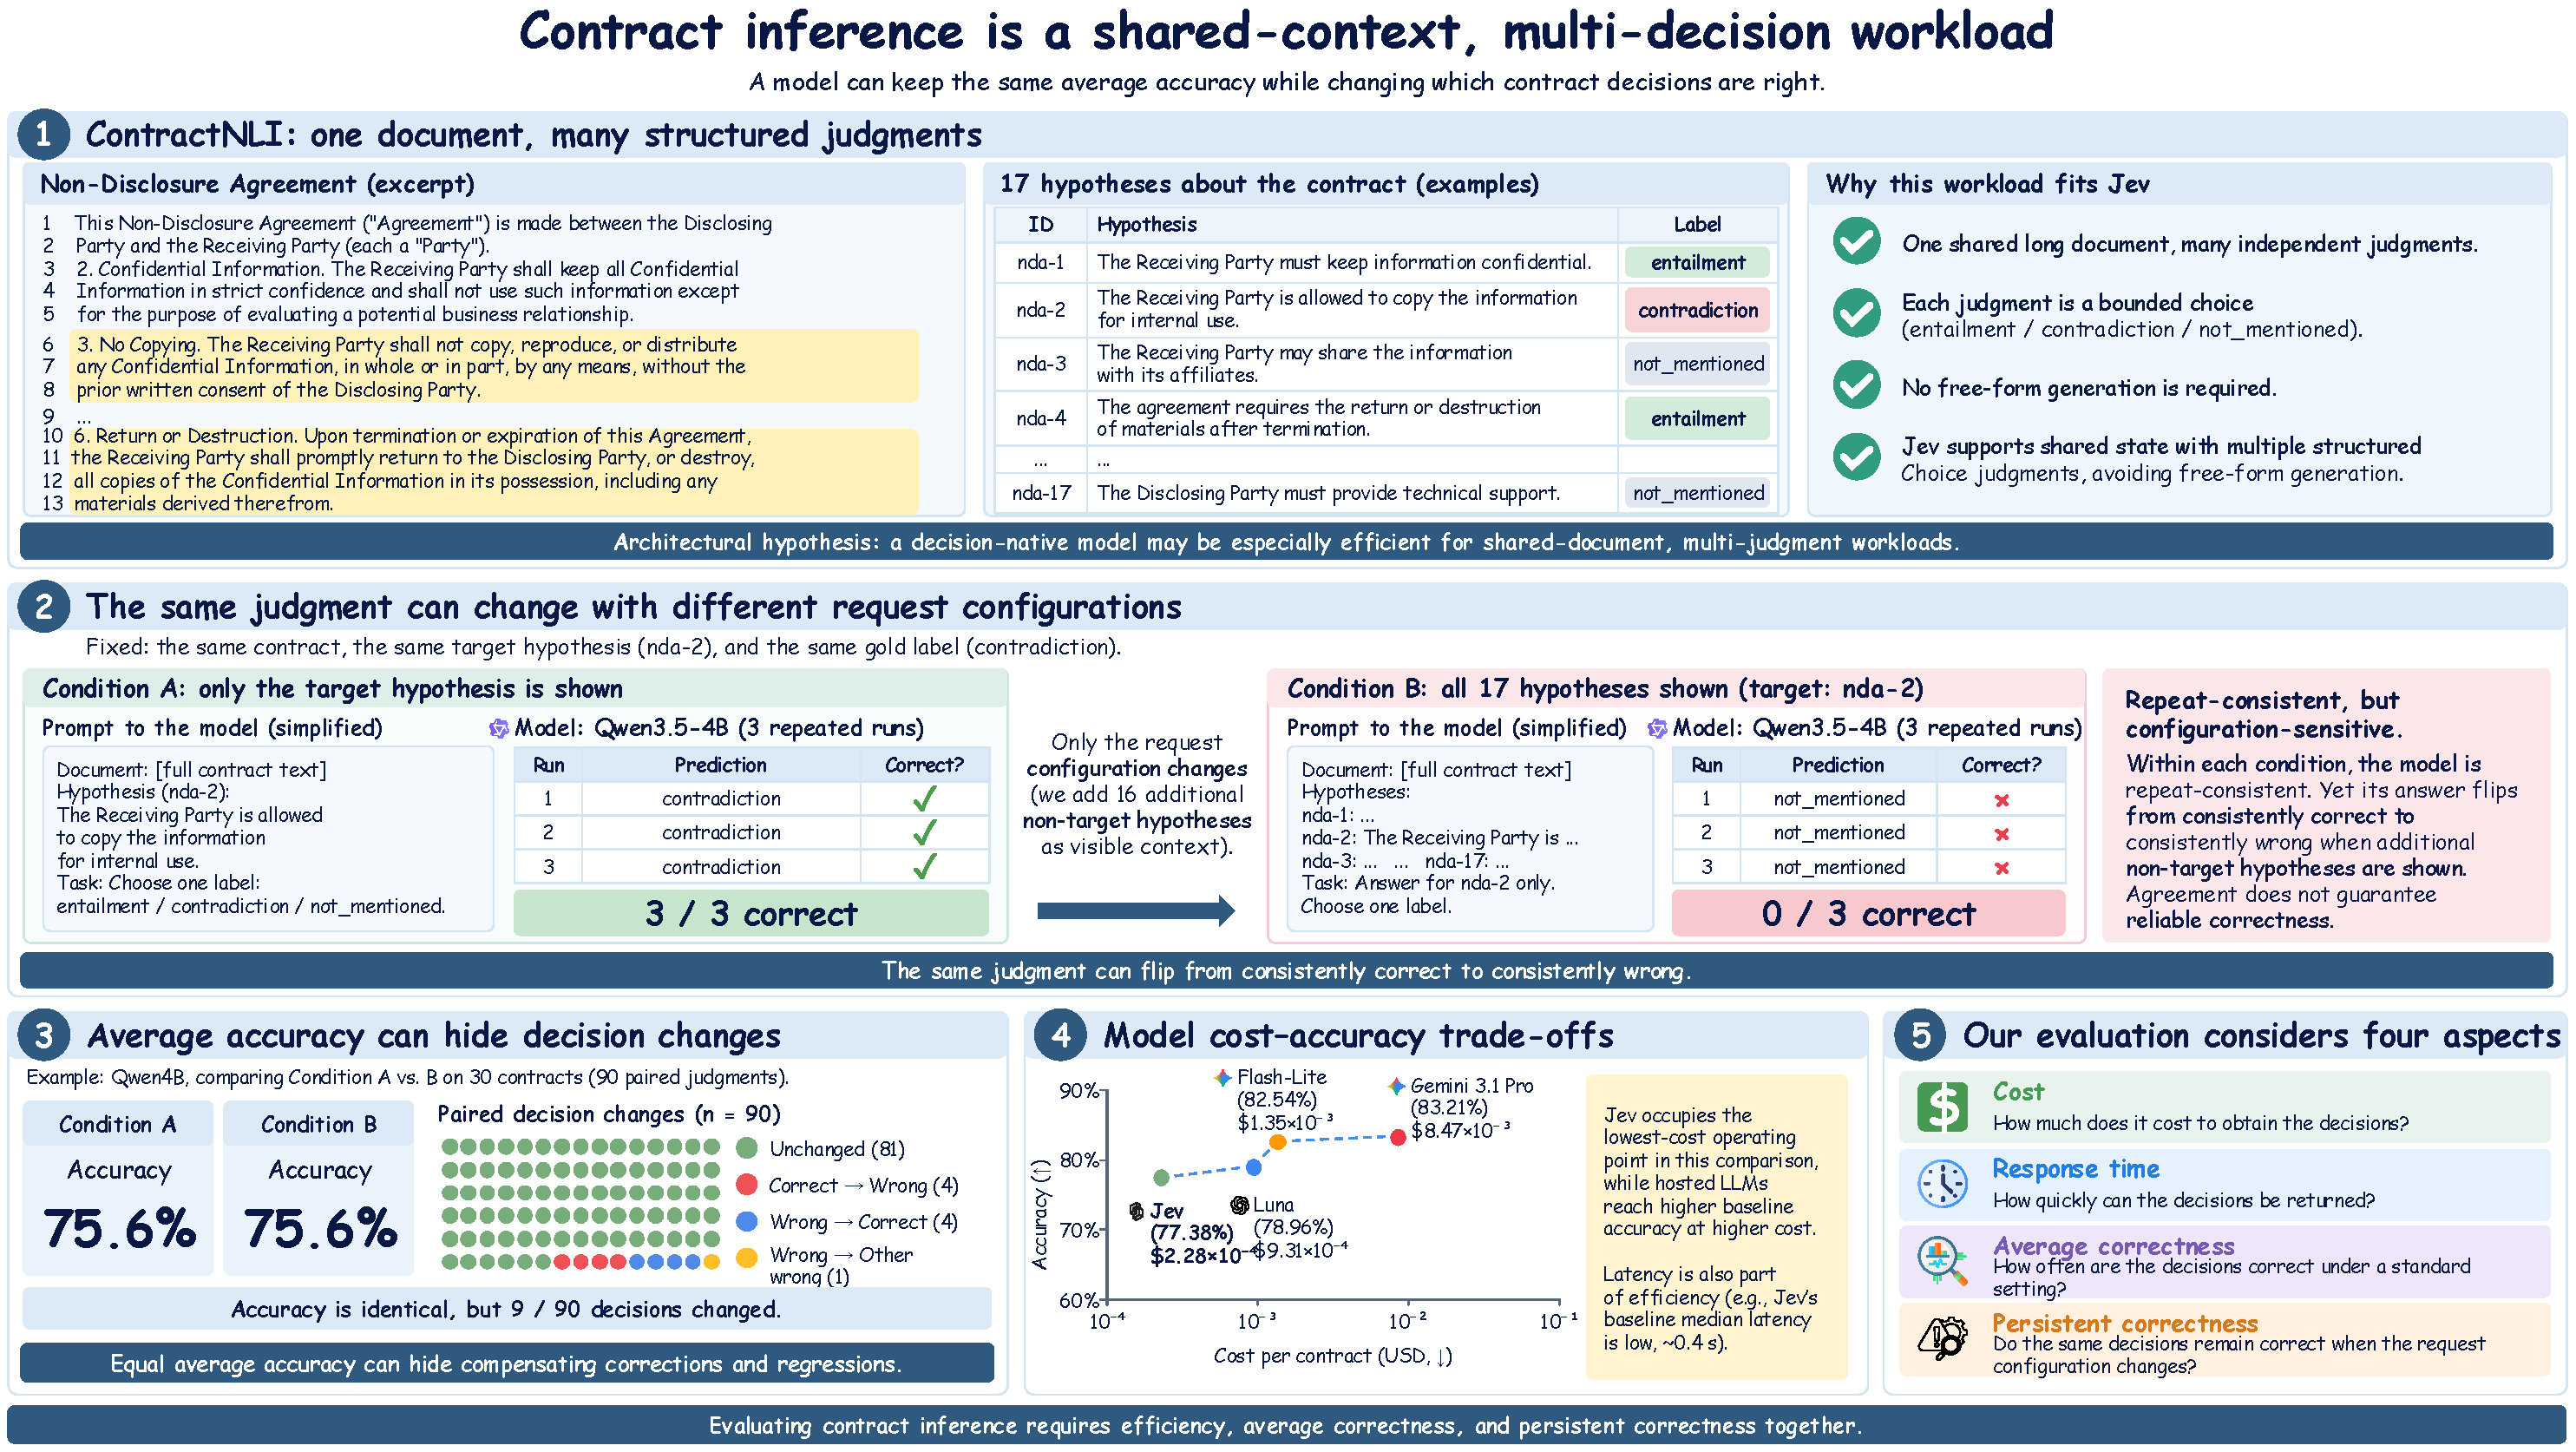
\includegraphics[width=\textwidth]{figures/contract_inference.pdf}
\caption[Overview of the contract-inference workload and evaluation questions.]{Overview of the evaluated workload and the questions studied. (1) ContractNLI poses many structured judgments about one shared document; hypotheses are paraphrased for illustration. (2) A fixed development-set judgment (contract 595, hypothesis nda-2) changes from consistently correct to consistently wrong when Qwen3.5-4B, with thinking disabled, sees additional non-target hypotheses; the contract, requested output, and inference settings remain unchanged. (3) On the test stability panel, Qwen3.5-4B has identical Condition A and B accuracy, yet nine of 90 paired judgments change. (4) Jev occupies the lowest-cost point among the compared models while hosted models reach higher baseline accuracy (Section~\ref{sec:test}). (5) We therefore evaluate cost, response time, average correctness, and persistent correctness together.
}
\label{fig:example}
\end{figure}

These considerations motivate a paired study of Jev and generative language models centered on three questions. \textbf{RQ1:} What trade-offs between cost, response time, and accuracy do Jev and its comparators exhibit? \textbf{RQ2:} Does higher accuracy imply that more judgments remain correct across repeated request conditions? \textbf{RQ3:} Which decisions change when visible hypotheses, requested outputs, or their order change? We address these questions by preserving target judgments and gold labels across controlled conditions, retaining invalid responses in the accuracy denominator, and estimating uncertainty at the contract level.

Our main evaluation uses the official ContractNLI test split for accuracy and a preselected subset for stability; all ten models complete both evaluations. Separate development analyses include earlier diagnostics that motivated the controlled design and additional comparisons collected after the test results were inspected. Three API comparators extend the original model selection using the same task, samples, and scoring rules.

Our contributions are:
\begin{itemize}[leftmargin=*,itemsep=2pt,topsep=3pt,parsep=0pt,partopsep=0pt]
\item A paired cost--accuracy evaluation of Jev and its comparators on fixed contract judgments, relating classification quality to response time and inference expenditure under explicit pricing assumptions (Sections~\ref{sec:task}--\ref{sec:test}).
\item An evaluation of average and persistent correctness that distinguishes their observed rankings and compares them on shared targets, with paired uncertainty estimates to define the scope of the conclusions (Section~\ref{sec:test}).
\item Controlled behavioral diagnostics that reveal compensating corrections and regressions, distinguish persistent correctness from stable errors, and interpret request sensitivity alongside repetition under unchanged conditions (Appendices~\ref{sec:diagnostics} and~\ref{sec:findings}--\ref{sec:planned}).
\end{itemize}

\section{Task and Evaluation Design}
\label{sec:task}
For a contract $d$, let $H_d=\{h_1,\ldots,h_{17}\}$ denote the original hypothesis set, with gold labels $y_{dh}\in\{\E,\C,\N\}$ for entailment, contradiction, and not mentioned. A model returns a label $\hat y_{dh}$ or no valid prediction. We evaluate ContractNLI's classification component; evidence-span extraction is outside the scope of this study. Every prediction is scored against the existing annotations, without new human labeling or model-based judging.

\paragraph{Accuracy and validity.}
The baseline requests all 17 labels jointly, once per contract. A valid response must contain exactly the requested IDs and one of the three allowed labels for each. Accuracy is computed over all intended judgments, with invalid responses counted as incorrect. We also report Macro-F1 and valid-response coverage. Responses that exhaust the generation allowance before producing final labels remain failures of the evaluated configuration (Appendix~\ref{app:budget}).

\paragraph{Controlled request conditions.}
The stability study fixes one target hypothesis, called the anchor, for each selected test contract. Four conditions preserve its contract and gold label:
\begin{description}
\item[A.] Only the anchor is visible; only its label is requested.
\item[B.] All 17 hypotheses are visible; only the anchor label is requested.
\item[C.] The same catalog is visible; all 17 labels are requested, anchor first.
\item[D.] The same catalog is visible; all 17 labels are requested, anchor last.
\end{description}
The catalog order is fixed in B/C/D. A--B changes visible hypotheses at a fixed requested answer set; B--C changes output workload and structure at fixed visible content; C--D changes requested output order and structure. Each condition is repeated three times. Primary scoring uses only the fixed anchor; the extra labels in C/D do not increase the number of primary targets.

\paragraph{Correctness across all twelve responses.}
An anchor is \emph{consistently correct} only when every response across the four conditions and three repeats gives the correct label. A \emph{stable error} consists of twelve valid, identical, but incorrect labels. The remaining outcomes consist of either twelve valid labels that change, or a set containing at least one invalid response. These mutually exclusive categories distinguish persistent correctness from agreement alone, with every selected anchor retained in the denominator. Within-condition repeat disagreement separately describes variation under unchanged requests.

We also compare average and persistent correctness on identical targets by averaging correctness over all 360 anchor responses, again counting invalid responses as incorrect. Unlike the broader baseline accuracy, this mean and all-twelve correctness concern the same targets. The mean weights every response equally; all-twelve correctness requires every response for a target to succeed. Their relationship therefore depends on how errors are distributed across targets and cannot be inferred from the mean alone.

\paragraph{Paired changes.}
For conditions $b$ and $c$, let $V_{bc}$ contain anchor--replicate pairs $(d,h,r)$ with valid predictions under both conditions. Their label-change rate is
\begin{equation*}
F(b,c)=\frac{\sum_{(d,h,r)\in V_{bc}}\I[\hat y^b_{dhr}\ne\hat y^c_{dhr}]}{|V_{bc}|}.
\end{equation*}
For these valid pairs, we report coverage and separate correct-to-wrong, wrong-to-correct, and wrong-to-different-wrong changes. With complete coverage, the accuracy difference is determined by corrections minus regressions, rather than by the total number of changed decisions. Unchanged-repeat disagreement supplies a reference for variation, but subtracting it from a condition difference would not identify a causal effect.

\section{Data and Experimental Protocol}
\label{sec:protocol}
\subsection{Data and uncertainty}
The official ContractNLI test split contains 123 contracts and 2,091 judgments: 968 entailments, 220 contradictions, and 903 not-mentioned labels~\citep{koreeda2021contractnli}. We preserve full contract text, all original hypotheses, and their annotations. Evidence spans are excluded from model inputs. The stability panel selects 30 test contracts and one anchor per contract using seed 20260922 and document-specific anchor seeds, independently of labels and model predictions. The panel is a subset of the accuracy evaluation, so these are complementary analyses of overlapping contracts.

Each model receives 123 requests in the accuracy evaluation and 360 in the stability evaluation. The latter yields 90 primary judgments per condition from 30 independent contract targets. We estimate uncertainty using 5,000 whole-contract bootstrap resamples with seed 20260922, preserving paired observations when comparing models. The resulting intervals are descriptive and unadjusted for multiple comparisons~\citep{dror2018hitchhiker}. Repeated requests supply additional observations of the same contracts, rather than additional independent contracts.

The task, test inputs, target selection, and scoring rules were fixed before test inference. The configurations for Jev, both Qwen models, both Gemini models, Luna, and Astra were fixed before their respective test evaluations. Sonnet, Haiku, and Terra were added after inspecting earlier results; their configurations were fixed before collecting their test predictions, and they use the same samples and evaluation rules. The ten-model comparison therefore does not constitute a wholly prospective model selection. The development experiments use separate contracts and are analyzed separately; their later extension follows inspection of the test results (Appendix~\ref{app:development-protocol}).

\subsection{Models and inference}
We compare Jev 1.13.0 with Qwen3.5-4B and 9B, Gemini 3.5 Flash-Lite and 3.1 Pro Preview, GPT-5.6 Luna and Terra, GPT-6 Astra, Claude Sonnet 5, and Claude Haiku 4.5. Jev receives the contract as shared state and each requested hypothesis as a native Choice question. Generative models receive semantically aligned classification instructions and return a JSON label map. The baseline and controlled catalog prompts differ, but each is fixed across its corresponding comparisons. Appendix~\ref{app:repro} gives the classification instruction.

Flash-Lite uses minimal thinking, Gemini Pro low thinking, Luna no reasoning, and Astra high reasoning. Terra uses medium reasoning with a 16,384-token output allowance. Sonnet uses adaptive thinking with medium effort and the same allowance; Haiku disables thinking with an 8,192-token allowance. The three added models are accessed through a common third-party gateway, whereas Luna and Astra use their original OpenRouter route. These provider-specific operating points do not equalize computation or actual reasoning length.

Both Qwen test configurations use BF16, enabled thinking, temperature 1, top-$p$ 0.95, and a shared allowance of 32,768 tokens for reasoning and the final answer. They use native model templates, one GPU per model, and no separate reasoning cutoff. Their historical development configurations disable thinking; a paired development comparison in Appendix~\ref{app:fairness} examines the complete configuration change. No test prompts or settings are selected from model performance.

Requests are issued sequentially for each model, while different models may run concurrently. Stability conditions and repetitions are shuffled within each contract using the fixed schedule. No failed evaluation attempt is repaired, replaced, or automatically retried. Model-specific response interfaces remain part of the evaluated configuration. In particular, Jev's C/D intervention changes question-key order; it is not equivalent to an autoregressive output-position intervention, and requested output order need not match internal reasoning order.

\subsection{Cost and timing}
Quality and cost are measured over the same requests, including failed attempts. For Luna and Astra, API costs use provider-reported charges; for other API models, we multiply recorded token usage by the public input, output, and cache prices applicable to the evaluation. When usage is missing, its cost remains unknown, and we report the known subtotal and coverage separately. Baseline cost is averaged over the 123 baseline contracts; stability cost is reported separately for its 360 requests.

For each local model, rental-equivalent baseline cost is
\begin{equation}
\widehat C_{\mathrm{GPU}}=\frac{r}{123\times3600}\sum_{d=1}^{123}t_d,
\end{equation}
where $t_d$ is the measured request time and $r$ is \$2.00 per GPU-hour. Each model uses one GPU. This is a valuation of observed local inference time, not a measured bill or a claim about cloud throughput. The declared reference rate and hardware differences are documented in Appendix~\ref{app:development-protocol}; loading, idle allocation, storage, transfer, and taxes are excluded. Latency also reflects network, scheduling, caching, and provider infrastructure. An observed cost--accuracy frontier therefore describes these measured configurations and pricing assumptions.

Response time uses recorded client elapsed time, including request preparation, connection establishment, network transfer, service-side processing, and response validation. All test collections use the same client machine, with one in-flight request per model and no retries. We report the median and 95th percentile (P95), retaining failed attempts. These measurements describe the evaluated deployments; separate model computation, queueing time, and time to first token were not recorded.

\section{Results on the Official Test Split}
\label{sec:test}
The official-test comparison separates four aspects of performance: inference expenditure, response time, baseline accuracy, and correctness across repeated conditions. All ten models complete the 123-contract baseline and the 30-contract stability panel, with failed requests retained in the intended denominators. Figure~\ref{fig:jev-main-results} summarizes the comparison, and Tables~\ref{tab:testbaseline} and~\ref{tab:teststates} detail baseline and repeated-target correctness. Appendix~\ref{app:testdetails} provides condition-level scores and paired uncertainty.

\begin{figure*}[t]
\centering
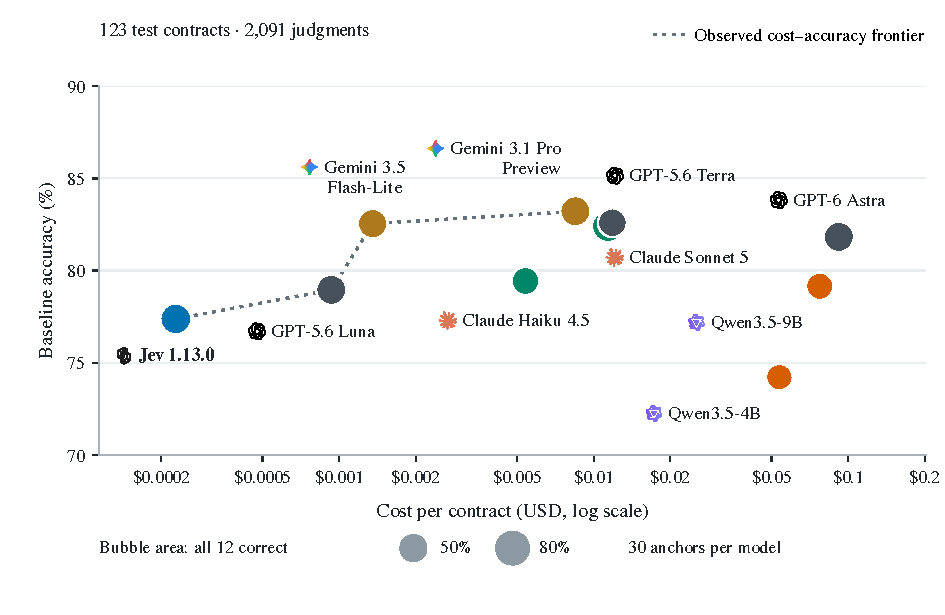
\includegraphics[width=0.92\textwidth]{figures/jev_test_cost_accuracy.pdf}
\caption[Official-test cost, accuracy, and correctness across all twelve responses.]{Jev 1.13.0 occupies the lowest-cost end of this comparison, while Gemini 3.1 Pro Preview attains the highest baseline accuracy. Coordinates summarize 123 official-test contracts (2,091 judgments); bubble area gives the fraction of 30 preselected anchors in distinct test contracts answered correctly in all four conditions and three repeats. All 360 planned stability requests per model enter the evaluation, and invalid responses cannot satisfy All 12 correct. The dotted frontier connects nondominated point estimates under the cost accounting in Section~\ref{sec:protocol}. Tables~\ref{tab:testbaseline} and~\ref{tab:testanchor} report confidence intervals; the connecting segments do not represent intermediate configurations or significant differences.
}
\label{fig:jev-main-results}
\end{figure*}

\begin{table*}[t]
\centering
\small
\setlength{\tabcolsep}{3pt}
\begin{tabularx}{\textwidth}{Xrrrrrr}
\toprule
\rowcolor{tableHeader}
Model & \shortstack{Accuracy\\(\%) $\uparrow$} & \shortstack{95\%\\interval} & \shortstack{Macro-F1\\(\%) $\uparrow$} & \shortstack{Cost\\(USD/contract) $\downarrow$} & \shortstack{Median\\time (s) $\downarrow$} & \shortstack{Valid\\calls} \\
\midrule
\rowcolor{jevRow}
\modelicon{jev}Jev 1.13.0 & 77.38 & [75.99, 78.81] & 72.23 & \bestscore{0.000228} & \bestscore{1.24} & 123/123 \\
\addlinespace[3pt]
\modelicon{gemini}Gemini 3.5 Flash-Lite & 82.54 & [81.11, 83.98] & 76.96 & 0.001353 & \secondscore{1.60} & 123/123 \\
\modelicon{gemini}Gemini 3.1 Pro Preview & \bestscore{83.21} & [81.68, 84.79] & \bestscore{77.71} & 0.008474 & 3.73 & 123/123 \\
\addlinespace[3pt]
\modelicon{openai}GPT-5.6 Luna & 78.96 & [77.19, 80.63] & 73.77 & \secondscore{0.000931} & 1.74 & 123/123 \\
\modelicon{openai}GPT-5.6 Terra & \secondscore{82.59} & [81.16, 84.03] & \secondscore{77.23} & 0.011839 & 11.61 & 123/123 \\
\modelicon{openai}GPT-6 Astra & 81.83 & [80.20, 83.36] & 76.55 & 0.091890 & 20.94 & 123/123 \\
\addlinespace[3pt]
\modelicon{claude}Claude Haiku 4.5 & 79.44 & [77.81, 81.11] & 74.46 & 0.005396 & 5.65 & 123/123 \\
\modelicon{claude}Claude Sonnet 5 & 82.40 & [80.97, 83.84] & 76.38 & 0.011352 & 3.27 & 123/123 \\
\addlinespace[3pt]
\modelicon{qwen}Qwen3.5-4B & 74.22 & [70.59, 77.38] & 71.67 & 0.053653 & 86.87 & 117/123 \\
\modelicon{qwen}Qwen3.5-9B & 79.15 & [76.81, 81.21] & 74.57 & 0.077361 & 134.64 & 122/123 \\
\bottomrule
\end{tabularx}
\caption{Official-test baseline: 123 contracts and 2,091 judgments per model. Failed requests remain incorrect; cost and median client response time include all 123 attempts. Accuracy intervals use 5,000 whole-contract bootstrap samples, without multiplicity adjustment. Section~\ref{sec:protocol} defines cost and timing. $\uparrow$/$\downarrow$: higher/lower is better. \textbf{Bold} and \underline{underlining} mark the best and second-best distinct values in columns with arrows, including ties; these marks do not imply statistical significance.}
\label{tab:testbaseline}
\end{table*}


\subsection{RQ1: Cost, response time, and accuracy}
Jev achieves 77.38\% accuracy at \$0.000228 per contract. All seven hosted language-model comparators have higher accuracy point estimates, ranging from 78.96\% for Luna to 83.21\% for Gemini Pro. Flash-Lite gains 5.16 percentage points over Jev at approximately six times the cost. The strength of evidence for these gains differs: the paired 95\% interval is 3.49--6.98 points for Flash-Lite minus Jev, but $-0.05$--3.11 points for Luna minus Jev (Appendix~\ref{app:testdetails}). Thus, the higher observed scores do not establish a reliable improvement for every comparator.

Under the stated prices, Jev, Luna, Flash-Lite, and Gemini Pro form the observed cost--accuracy frontier. The three added comparators broaden model-family coverage without extending this two-dimensional frontier. Sonnet and Terra achieve accuracy close to Flash-Lite at higher costs; Haiku falls between Jev and Flash-Lite in accuracy while costing more than either. The comparison is specific to these operating points and pricing bases. Qwen4B and Qwen9B achieve 74.22\% and 79.15\%, respectively, including six and one baseline requests that exhaust the generation allowance before producing final labels.

\paragraph{Cost increments and observed gains.}
Higher expenditure along the frontier does not yield a uniform return in accuracy. Gemini Pro costs 6.26 times as much as Flash-Lite for a gain of 0.67 percentage points, with a paired 95\% interval of $-0.72$--2.10 percentage points. It therefore has the highest accuracy point estimate, but no established advantage over Flash-Lite on this sample. Its all-twelve-correct count also exceeds Flash-Lite's by only one target. Frontier membership describes the observed cost and quality coordinates; paired uncertainty indicates how strongly the sample supports a difference. Together, they inform model choice without identifying a universally preferred configuration.

\paragraph{Response time and output workload.}
Jev also has the lowest observed median baseline response time: 1.24 seconds, compared with 1.60 for Flash-Lite and 1.74 for Luna. Their P95 times are 1.59, 2.78, and 2.25 seconds, respectively. The full comparison, including slower reasoning-enabled configurations and failed attempts, appears in Appendix~\ref{app:timing}.

At a fixed visible catalog of 17 hypotheses, requesting 17 labels instead of one (B--C) changes Jev's median response time from 1.15 to 1.22 seconds, versus 0.99 to 1.86 for Flash-Lite and 1.10 to 1.78 for Luna. This small increase describes the observed service behavior. It does not identify internal parallelism: fixed network overhead and serving policies can also affect the increase. Accuracy and latency must both be considered when choosing a request configuration.

Pairing requests by contract and repeat gives a median B--C increase of 0.19 seconds for Jev (descriptive 95\% interval: 0.06--0.24), 0.49 for Flash-Lite (0.45--0.58), and 0.67 for Luna (0.59--0.71). These summarize individual time differences, not differences between condition medians; intervals preserve all repeats within contracts. Rankings depend on the requested outputs: Flash-Lite has a lower median than Jev in B, whereas Jev has the lower median for joint prediction. Speed comparisons therefore require a specified workload.

\subsection{RQ2: Correctness across repeated conditions}
\begin{table*}[t]
\centering
\small
\begin{tabularx}{\textwidth}{Xrrrrr}
\toprule
\rowcolor{tableHeader}
Model & \shortstack{Mean correct\\(\%) $\uparrow$} & \shortstack{All 12\\correct $\uparrow$} & \shortstack{Same\\wrong} & \shortstack{Changed\\valid} & \shortstack{Any\\invalid} \\
\midrule
\rowcolor{jevRow}
\modelicon{jev}Jev 1.13.0 & 79.44 & \secondscore{23/30} & 5 & 2 & 0 \\
\addlinespace[3pt]
\modelicon{gemini}Gemini 3.5 Flash-Lite & 82.50 & 21/30 & 4 & 5 & 0 \\
\modelicon{gemini}Gemini 3.1 Pro Preview & \secondscore{85.28} & 22/30 & 2 & 5 & 1 \\
\addlinespace[3pt]
\modelicon{openai}GPT-5.6 Luna & 81.94 & 22/30 & 3 & 5 & 0 \\
\modelicon{openai}GPT-5.6 Terra & 80.56 & 20/30 & 2 & 8 & 0 \\
\modelicon{openai}GPT-6 Astra & 76.39 & 22/30 & 6 & 2 & 0 \\
\addlinespace[3pt]
\modelicon{claude}Claude Haiku 4.5 & 81.94 & 19/30 & 2 & 9 & 0 \\
\modelicon{claude}Claude Sonnet 5 & \bestscore{86.67} & \bestscore{24/30} & 1 & 5 & 0 \\
\addlinespace[3pt]
\modelicon{qwen}Qwen3.5-4B & 77.50 & 17/30 & 2 & 8 & 3 \\
\modelicon{qwen}Qwen3.5-9B & 79.17 & 18/30 & 2 & 8 & 2 \\
\bottomrule
\end{tabularx}
\caption{Mean correctness scores the same 30 test anchors across four conditions and three repeats (360 judgments); invalid responses count wrong. All 12 correct requires every answer to be correct. Remaining anchors have twelve identical wrong labels, twelve valid but changing labels, or an invalid response; invalidity takes precedence. The four outcome counts sum to 30. \textbf{Bold}/\underline{underlining} mark the best/second-best distinct values in arrowed columns; they do not indicate significance.}
\label{tab:teststates}
\end{table*}

Sonnet keeps 24 of 30 anchors correct across all twelve responses, followed by Jev with 23. Gemini Pro, Luna, and Astra each retain 22, while Qwen9B retains 18 (Table~\ref{tab:teststates}). The Sonnet--Jev difference amounts to one target, with a paired 95\% interval of $-10.00$--16.67 percentage points; the panel therefore does not establish a general stability advantage for the comparison with Sonnet. Jev exceeds Haiku, Qwen9B, and Qwen4B by four, five, and six targets, respectively. The paired intervals exclude zero for Haiku and Qwen4B, while Qwen9B's interval reaches zero. These unadjusted comparisons remain exploratory.

\paragraph{Similar means on the same targets.}
Baseline accuracy and all-twelve correctness yield different observed rankings, but their target sets differ. To hold target composition fixed, Table~\ref{tab:teststates} compares mean and persistent correctness within the stability panel. Jev answers 286 of its 360 anchor responses correctly (79.44\%), and Qwen9B answers 285 (79.17\%). These nearly identical means coexist with 23 versus 18 anchors that remain correct throughout. The paired mean difference, Qwen9B minus Jev, is $-0.28$ points (95\% interval: $-9.44$--10.00), which does not establish equivalence. The comparison nevertheless shows that the difference in persistent-correctness point estimates remains when both measures use identical targets.

\paragraph{The distribution of errors matters.}
The allocation of errors across targets explains this distinction. Jev has five anchors that receive the same wrong label throughout and two whose labels change. Qwen9B has two targets with consistently wrong labels, eight targets with changing valid labels, and two targets with invalid responses. Similar totals of correct responses can therefore leave different numbers of targets correct throughout. Agreement alone obscures another part of the comparison: Jev and Astra each repeat the same label on 28 of 30 targets, compared with Sonnet's 25. However, five of Jev's and six of Astra's consistent labels are wrong, compared with one for Sonnet. Treating agreement as successful stability would reverse the interpretation of these outcomes.

\subsection{RQ3: Changes hidden by average accuracy}
\begin{figure*}[t]
\centering
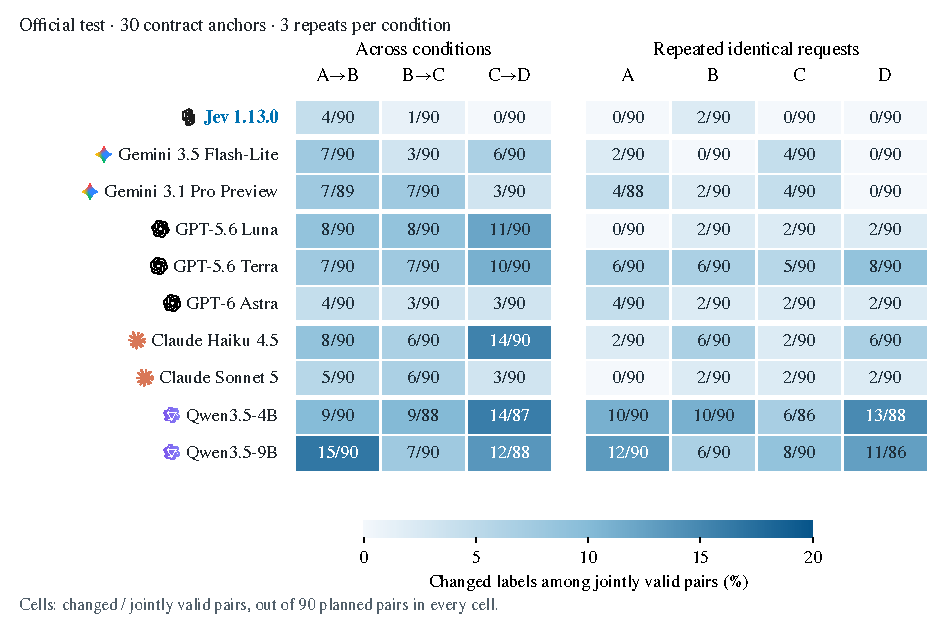
\includegraphics[width=0.82\textwidth]{figures/test_sensitivity.pdf}
\caption[Official-test changes across conditions and identical-request repetition.]{Label changes occur both across request conditions and under identical-request repetition. Results cover 30 preselected official-test contracts, with one anchor per contract and three repeats per condition. Cells show changed labels over jointly valid pairs; color encodes the corresponding percentage. Across-condition comparisons match the same anchor and repeat, while repetition cells use all three unordered repeat pairs per anchor, giving 90 planned pairs in every cell. A exposes and requests only the anchor; B exposes all hypotheses but requests the anchor; C requests all labels with the anchor first; D places it last. Invalid responses are excluded from these pairwise percentages, with the valid denominator shown in each cell, but count as incorrect in the accuracy and All 12 correct evaluations. All ten models complete the planned stability collection. A changed answer may improve or worsen correctness, so these rates do not measure performance degradation.
}
\label{fig:test-sensitivity}
\end{figure*}
Condition-level accuracy can remain unchanged even when the underlying decisions differ. For Qwen4B, A and B have identical accuracy, yet nine of 90 paired responses change: four regressions, four corrections, and one switch between wrong labels. Terra likewise has equal accuracy in B and C despite seven changed responses, comprising three regressions, three corrections, and one wrong-label switch. In both cases, the contract and target remain fixed, while opposing changes cancel in the aggregate score.

Sensitivity to requested output order also varies across configurations. Haiku changes 14 of 90 paired responses from C to D, including twelve regressions and two corrections. Its accuracy falls by 11.11 percentage points (descriptive paired 95\% interval: $-23.33$ to $-1.11$). Jev shows no C--D changes in this panel, although its question-key intervention differs from autoregressive output ordering and a finite sample with no changes does not establish invariance. Appendix~\ref{app:testdetails} reports all transition counts and valid-pair coverage, retaining failures separately from valid label changes.

\paragraph{Variation without a changed condition.}
Unchanged-request repetition shows why cross-condition changes require a reference for variability. In Figure~\ref{fig:test-sensitivity}, Qwen9B changes 15 of 90 valid pairs between A and B, alongside 12 of 90 repeat pairs within A and six of 90 within B. Its C--D comparison changes 12 of 88 valid pairs, while repeats within D change eleven of 86 valid pairs. Thus, variation is already present without altering the request condition. Because these counts describe different dependent comparisons, subtracting them would not estimate the causal contribution of an intervention. Directional transitions, unchanged-repeat variation, and invalid-response coverage together clarify what a single change rate leaves unresolved.

\subsection{Can incomplete answers explain the differences?}
Generation-budget exhaustion lowers the Qwen scores, but cannot fully account for their difference from Flash-Lite. To bound the numerical effect of missing labels, we assign every missing label in a truncated baseline response its correct answer while holding all observed answers fixed. This deliberately optimistic calculation raises Qwen4B from 74.22\% to at most 79.10\% and Qwen9B from 79.15\% to at most 79.96\%, both below Flash-Lite's observed 82.54\%. These bounds do not replace the reported scores or predict what a larger generation allowance would achieve.

The anchor outcomes show that errors in completed answers also limit persistent correctness. Both Qwen9B targets with an invalid response already contain wrong answers among their other eleven responses: four for one target and one for the other. Correcting the two missing answers would therefore leave its all-twelve-correct count at 18. For Qwen4B, only two of the three affected targets have all remaining responses correct. Correct answers for all missing responses could raise its count from 17 to at most 19, still below Jev's 23. The difference thus cannot be attributed solely to retaining truncated responses in the evaluation. Appendix~\ref{app:budget} gives the termination evidence and scoring rationale.

\section{Development Diagnostics}
\label{sec:development-overview}
Development experiments provide separate diagnostics under their original samples and settings (Appendices~\ref{sec:diagnostics}--\ref{sec:planned}). Qwen4B changes 87 of 510 labels between joint and single-hypothesis requests, while its correct count changes by only four. In the disjoint anchor panel, A and B have equal accuracy but 24 of 90 responses change: twelve corrections and twelve regressions. Unchanged repeats within each arm agree, and Figure~\ref{fig:example} shows one regression.

A paired Qwen configuration comparison also finds higher mean correctness without a clear gain in all-twelve correctness, despite much greater token use. Reasoning, sampling, and output allowance change together; Appendix~\ref{app:fairness} reports the full comparison. These diagnostics motivate separating changes in visible hypotheses, requested outputs, and inference settings.

\section{Related Work}
\label{sec:related}
\paragraph{Legal-task evaluation.}
ContractNLI, CUAD, and LegalBench evaluate contract inference, evidence extraction, and broader legal reasoning~\citep{koreeda2021contractnli,hendrycks2021cuad,guha2023legalbench}. We use ContractNLI's existing labels to examine how request configuration affects multiple judgments about one document.

\paragraph{Request sensitivity and behavioral evaluation.}
Prompt studies reveal sensitivity to demonstration order and meaning-preserving formatting~\citep{lu2022fantastically,sclar2024quantifying}. Batch prompting examines efficiency and positional effects across jointly requested examples~\citep{cheng2023batchprompting,lin2024batchprompt}; related work varies evidence location and answer-option order~\citep{liu2024lost,zheng2024selectors}. Our controls vary visible hypotheses, requested outputs, and output order while holding the contract and target fixed. CheckList motivates behavioral analysis beyond average accuracy~\citep{ribeiro2020checklist}, and order-consistent scoring shows that similar ranking quality can coexist with different decisions~\citep{frohmann2026equal}. We distinguish corrections, regressions, persistent errors, and variation across repeats under unchanged conditions.

\paragraph{Joint quality and cost evaluation.}
HELM jointly evaluates quality, robustness, and efficiency~\citep{liang2023helm}, while model routing studies accuracy--cost trade-offs~\citep{chen2024frugalgpt,ong2025routellm}. We compare individual configurations with explicit costs and invalid-response accounting, connecting average correctness to whether fixed judgments remain correct across repeated conditions. Appendix~\ref{app:related} details these comparisons and additional legal, prompting, and evaluation literature.

\section{Discussion and Conclusion}
\label{sec:conclusion}
Cost, response time, average accuracy, and persistent correctness describe complementary aspects of contract inference. Jev has the lowest cost and median baseline response time among the evaluated configurations, while hosted language models achieve higher baseline accuracy. Gemini Pro and Sonnet have the highest baseline and all-twelve-correct point estimates, respectively. Jev is competitive on repeated-condition correctness, but the small anchor panel does not establish a general stability advantage. The cost frontier remains specific to the evaluated configurations and prices.

Decision-level analysis explains these distinctions. On identical targets, similar mean correctness can coexist with different numbers of judgments that remain correct throughout. Corrections and regressions can cancel each other out in aggregate accuracy, while agreement can preserve errors. Even optimistically completing truncated answers leaves both Qwen configurations below Flash-Lite in baseline accuracy and below Jev in all-twelve correctness. Reporting correctness, direction of change, and validity alongside expenditure thus clarifies the observed trade-offs.

\label{sec:content-end}
\clearpage
\section*{Limitations}
\label{sec:limitations}
The official test contains 123 contracts and a stability subset of 30 contract targets, all drawn from the same 17 hypothesis types. The development analyses use 30 contracts for grouping experiments and ten different contracts for anchor controls. These samples limit generalization to other legal questions and domains. We use existing annotations without a human performance comparison, new adjudication, or external-domain validation. An official held-out split does not establish absence from model training data.

The two principal quality measures use different target sets: baseline accuracy spans every contract--hypothesis pair, whereas all-twelve correctness concerns one anchor in each selected contract. Ranking differences can therefore reflect both target composition and sensitivity to the tested conditions. Three repeats provide limited information about possible responses, and bootstrap intervals may degenerate when no changes are observed. The small stability panel makes rankings sensitive to a few targets. Its intervals and paired comparisons are descriptive and not corrected for multiple testing.

Inference settings, interfaces, instruction wording, hardware, providers, and collection times differ across models. Hosted models may change behind a fixed identifier. Jev's question-key ordering differs from autoregressive output ordering. The Qwen development comparison changes reasoning, temperature, and generation allowance together, so it cannot isolate the effect of reasoning alone. Nor does a common token limit equalize realized computation. Budget-exhausted answers are failures of the evaluated configuration, rather than evidence that a task is intrinsically beyond the model.

Costs follow the calculation in Section~\ref{sec:protocol}. Local GPU costs use a declared rental equivalent. Local estimates exclude loading, idle allocation, and other non-inference expenditure, and do not measure cloud throughput. Latency includes infrastructure and network effects. The frontier may change under other prices, serving methods, or reasoning budgets.

Latency comparisons use one client but different collection times, providers, routes, and inference settings, with uncontrolled provider caching. Small differences in client-side preparation also remain. They cannot isolate architecture-level efficiency, separate computation from network and queueing delays, or establish throughput under concurrent load.

The model comparison developed in stages: Sonnet, Haiku, and Terra were added after earlier results were inspected. Their predictions use fixed task and scoring rules, but model selection itself is exploratory. All ten test stability evaluations are complete; historical Astra development anchor coverage remains incomplete and is analyzed separately. Broader evidence would be required to assess suitability for legal practice or financial decision-making.

\section*{Ethical considerations}
We use ContractNLI under its stated CC BY 4.0 license and retain attribution to its creators. The study uses existing data and annotations, with no new personal-data collection or human participation. Examples retain their dataset identifiers and original labels. Any redistribution should preserve attribution and licensing while minimizing additional identifying information. The evaluation concerns model behavior in a research setting. Incorrect or unstable judgments could cause harm if treated as professional legal or financial determinations.

\bibliography{references}

\clearpage
\appendix
\suppressfloats[t]
\makeatletter
\setlength{\@dblfptop}{0pt}
\setlength{\@dblfpsep}{18pt}
\setlength{\@dblfpbot}{0pt plus 1fil}
\makeatother

\section{Supplementary Official-Test Comparisons}
\label{app:testdetails}
The supplementary official-test analyses examine class-specific errors, paired model differences, and response transitions for all ten models. Both baseline and stability evaluations are complete. The following development appendices retain the earlier experiments and add baseline, repetition, order, and anchor comparisons; their samples and results remain separate from the official-test evaluation.

Table~\ref{tab:testanchor} gives condition-level correctness, all-twelve uncertainty, and response validity for the complete stability panel. Each model has 360 attempted requests, with 90 intended anchor responses per condition.
\begin{table*}[t]
\centering
\small
\begin{tabularx}{\textwidth}{Xrrrrcrr}
\toprule
\rowcolor{tableHeader}
Model & \shortstack{A (\%)\\$\uparrow$} & \shortstack{B (\%)\\$\uparrow$} & \shortstack{C (\%)\\$\uparrow$} & \shortstack{D (\%)\\$\uparrow$} & \shortstack{All 12\\correct $\uparrow$} & \shortstack{95\%\\interval} & Valid calls \\
\midrule
\rowcolor{jevRow}
\modelicon{jev}Jev 1.13.0 & 76.67 & 81.11 & 80.00 & 80.00 & \secondscore{23/30} & [60.0, 90.0] & 360/360 \\
\addlinespace[3pt]
\modelicon{gemini}Gemini 3.5 Flash-Lite & 82.22 & 83.33 & 84.44 & 80.00 & 21/30 & [53.3, 83.3] & 360/360 \\
\modelicon{gemini}Gemini 3.1 Pro Preview & \bestscore{85.56} & \bestscore{85.56} & 86.67 & \secondscore{83.33} & 22/30 & [56.7, 86.7] & 359/360 \\
\addlinespace[3pt]
\modelicon{openai}GPT-5.6 Luna & 80.00 & 82.22 & 84.44 & 81.11 & 22/30 & [56.7, 86.7] & 360/360 \\
\modelicon{openai}GPT-5.6 Terra & 76.67 & 83.33 & 83.33 & 78.89 & 20/30 & [50.0, 83.3] & 360/360 \\
\modelicon{openai}GPT-6 Astra & 76.67 & 74.44 & 75.56 & 78.89 & 22/30 & [56.7, 86.7] & 360/360 \\
\addlinespace[3pt]
\modelicon{claude}Claude Haiku 4.5 & 78.89 & \secondscore{84.44} & \secondscore{87.78} & 76.67 & 19/30 & [46.7, 80.0] & 360/360 \\
\modelicon{claude}Claude Sonnet 5 & \secondscore{83.33} & \secondscore{84.44} & \bestscore{88.89} & \bestscore{90.00} & \bestscore{24/30} & [63.3, 93.3] & 360/360 \\
\addlinespace[3pt]
\modelicon{qwen}Qwen3.5-4B & 75.56 & 75.56 & 81.11 & 77.78 & 17/30 & [40.0, 73.3] & 357/360 \\
\modelicon{qwen}Qwen3.5-9B & 78.89 & 80.00 & 78.89 & 78.89 & 18/30 & [43.3, 76.7] & 358/360 \\
\bottomrule
\end{tabularx}
\caption{Official-test stability evaluation on 30 contracts with one anchor each, four conditions and three repeats (90 anchor judgments per condition; 360 requests per model). All 360 requests were attempted for each of the ten models. All 12 correct retains all 30 targets and requires every response to be valid and correct. Its percentage intervals use 5,000 whole-contract bootstrap samples. Invalid responses remain in every intended denominator. $\uparrow$/$\downarrow$: higher/lower is better. \textbf{Bold} and \underline{underlining} mark the best and second-best distinct values in columns with arrows, including ties; these marks do not imply statistical significance.}
\label{tab:testanchor}
\end{table*}


Table~\ref{tab:testclassrecalls} reports class recalls for all ten models on the same 123 test contracts. Table~\ref{tab:testpaired} reports paired differences from Jev for baseline accuracy and correctness across all twelve responses. Table~\ref{tab:teststates} separates persistent correctness, stable errors, valid but changed answers, and invalid responses. Figure~\ref{fig:test-sensitivity} compares changes across conditions with disagreement under unchanged repetition; Table~\ref{tab:testchanges} separates the directions of those condition changes. These analyses retain the same contract clusters and intended denominators as the main evaluation.

The class recalls expose error profiles that overall accuracy obscures. Jev has the highest observed contradiction recall, Astra the highest entailment recall, and Sonnet the highest not-mentioned recall. These descriptive comparisons concern classes with unequal support; they do not establish significant differences between models.

Jev correctly classifies 170 of 220 contradictions, whereas Gemini Pro correctly classifies 135. Relative to Jev, Gemini Pro gains 47 correct entailments and 110 correct not-mentioned labels but loses 35 correct contradictions, producing its net gain of 122 correct judgments. Overall accuracy weights class-specific recall by class support. These counts do not establish an application-specific preference without an independently justified valuation of the errors.

Qwen9B illustrates how similar condition-level scores can conceal changes at the target level. Each condition yields 71 or 72 correct answers among 90 intended judgments, yet eight targets receive different valid labels across the twelve responses. Two more targets encounter generation-budget exhaustion, and two repeat the same wrong label throughout. The remaining eighteen are correct in every response. Invalid answers count as incorrect and prevent all-twelve correctness, but supply no observed label for the change-rate calculation.

\begin{table*}[t]
\centering
\small
\begin{tabularx}{\textwidth}{Xrrr}
\toprule
\rowcolor{tableHeader}
Model & \shortstack{Entailment recall\\(\%) $\uparrow$ $n=968$} & \shortstack{Contradiction recall\\(\%) $\uparrow$ $n=220$} & \shortstack{Not mentioned recall\\(\%) $\uparrow$ $n=903$} \\
\midrule
\rowcolor{jevRow}
\modelicon{jev}Jev 1.13.0 & 86.88 & \bestscore{77.27} & 67.22 \\
\addlinespace[3pt]
\modelicon{gemini}Gemini 3.5 Flash-Lite & 91.32 & 63.18 & 77.85 \\
\modelicon{gemini}Gemini 3.1 Pro Preview & 91.74 & 61.36 & \secondscore{79.40} \\
\addlinespace[3pt]
\modelicon{openai}GPT-5.6 Luna & \secondscore{93.29} & 73.64 & 64.89 \\
\modelicon{openai}GPT-5.6 Terra & 89.98 & 71.36 & 77.41 \\
\modelicon{openai}GPT-6 Astra & \bestscore{93.60} & \secondscore{74.55} & 70.99 \\
\addlinespace[3pt]
\modelicon{claude}Claude Haiku 4.5 & 91.63 & 62.73 & 70.43 \\
\modelicon{claude}Claude Sonnet 5 & 90.50 & 55.00 & \bestscore{80.40} \\
\addlinespace[3pt]
\modelicon{qwen}Qwen3.5-4B & 77.48 & 67.27 & 72.43 \\
\modelicon{qwen}Qwen3.5-9B & 84.61 & 73.64 & 74.64 \\
\bottomrule
\end{tabularx}
\caption{Class recalls on the official-test baseline: 123 contracts and all 2,091 labeled judgments per model. Header counts give the gold-label support for each class and are identical across all ten models. Failed requests contribute no correct predictions and remain in each class denominator. These are test-split results, separate from the development class analysis. $\uparrow$/$\downarrow$: higher/lower is better. \textbf{Bold} and \underline{underlining} mark the best and second-best distinct values in columns with arrows, including ties; these marks do not imply statistical significance.}
\label{tab:testclassrecalls}
\end{table*}



\begin{table*}[t]
\centering
\small
\begin{tabularx}{\textwidth}{Xrrrr}
\toprule
\rowcolor{tableHeader}
Model & $\Delta$ accuracy & 95\% interval & $\Delta$ All 12 correct & 95\% interval \\
\midrule
\modelicon{gemini}Gemini 3.5 Flash-Lite & +5.16 & [+3.49, +6.98] & -6.67 & [-16.67, +0.00] \\
\modelicon{gemini}Gemini 3.1 Pro Preview & +5.83 & [+4.11, +7.65] & -3.33 & [-16.67, +10.00] \\
\addlinespace[3pt]
\modelicon{openai}GPT-5.6 Luna & +1.58 & [-0.05, +3.11] & -3.33 & [-10.00, +0.00] \\
\modelicon{openai}GPT-5.6 Terra & +5.21 & [+3.73, +6.70] & -10.00 & [-20.00, +0.00] \\
\modelicon{openai}GPT-6 Astra & +4.45 & [+2.92, +5.93] & -3.33 & [-16.67, +10.00] \\
\addlinespace[3pt]
\modelicon{claude}Claude Haiku 4.5 & +2.06 & [+0.43, +3.73] & -13.33 & [-26.67, -3.33] \\
\modelicon{claude}Claude Sonnet 5 & +5.02 & [+3.25, +6.79] & +3.33 & [-10.00, +16.67] \\
\addlinespace[3pt]
\modelicon{qwen}Qwen3.5-4B & -3.16 & [-6.70, +0.00] & -20.00 & [-36.67, -3.33] \\
\modelicon{qwen}Qwen3.5-9B & +1.77 & [-0.43, +3.73] & -16.67 & [-33.33, +0.00] \\
\bottomrule
\end{tabularx}
\caption{Paired differences from Jev in percentage points (comparison model minus Jev). The baseline resamples 123 contracts and All 12 correct resamples 30 contracts, using 5,000 paired whole-contract bootstrap draws. All ten models have complete evaluations. Intervals are exploratory, descriptive, and unadjusted for multiple comparisons.}
\label{tab:testpaired}
\end{table*}

\begin{table*}[t]
\centering
\small
\begin{tabularx}{\textwidth}{Xlrrrrr}
\toprule
\rowcolor{tableHeader}
Model & Contrast & Valid pairs & Changed & C$\to$W & W$\to$C & W$\to$W \\
\midrule
\multirow[c]{3}{*}{\modelicon{jev}Jev 1.13.0} & A$\to$B & 90/90 & 4 & 0 & 4 & 0 \\
 & B$\to$C & 90/90 & 1 & 1 & 0 & 0 \\
 & C$\to$D & 90/90 & 0 & 0 & 0 & 0 \\
\addlinespace[3pt]
\multirow[c]{3}{*}{\modelicon{gemini}Gemini 3.5 Flash-Lite} & A$\to$B & 90/90 & 7 & 3 & 4 & 0 \\
 & B$\to$C & 90/90 & 3 & 1 & 2 & 0 \\
 & C$\to$D & 90/90 & 6 & 5 & 1 & 0 \\
\multirow[c]{3}{*}{\modelicon{gemini}Gemini 3.1 Pro Preview} & A$\to$B & 89/90 & 7 & 4 & 3 & 0 \\
 & B$\to$C & 90/90 & 7 & 3 & 4 & 0 \\
 & C$\to$D & 90/90 & 3 & 3 & 0 & 0 \\
\addlinespace[3pt]
\multirow[c]{3}{*}{\modelicon{openai}GPT-5.6 Luna} & A$\to$B & 90/90 & 8 & 3 & 5 & 0 \\
 & B$\to$C & 90/90 & 8 & 3 & 5 & 0 \\
 & C$\to$D & 90/90 & 11 & 6 & 3 & 2 \\
\multirow[c]{3}{*}{\modelicon{openai}GPT-5.6 Terra} & A$\to$B & 90/90 & 7 & 0 & 6 & 1 \\
 & B$\to$C & 90/90 & 7 & 3 & 3 & 1 \\
 & C$\to$D & 90/90 & 10 & 6 & 2 & 2 \\
\multirow[c]{3}{*}{\modelicon{openai}GPT-6 Astra} & A$\to$B & 90/90 & 4 & 3 & 1 & 0 \\
 & B$\to$C & 90/90 & 3 & 1 & 2 & 0 \\
 & C$\to$D & 90/90 & 3 & 0 & 3 & 0 \\
\addlinespace[3pt]
\multirow[c]{3}{*}{\modelicon{claude}Claude Haiku 4.5} & A$\to$B & 90/90 & 8 & 1 & 6 & 1 \\
 & B$\to$C & 90/90 & 6 & 0 & 3 & 3 \\
 & C$\to$D & 90/90 & 14 & 12 & 2 & 0 \\
\multirow[c]{3}{*}{\modelicon{claude}Claude Sonnet 5} & A$\to$B & 90/90 & 5 & 2 & 3 & 0 \\
 & B$\to$C & 90/90 & 6 & 1 & 5 & 0 \\
 & C$\to$D & 90/90 & 3 & 0 & 1 & 2 \\
\addlinespace[3pt]
\multirow[c]{3}{*}{\modelicon{qwen}Qwen3.5-4B} & A$\to$B & 90/90 & 9 & 4 & 4 & 1 \\
 & B$\to$C & 88/90 & 9 & 1 & 7 & 1 \\
 & C$\to$D & 87/90 & 14 & 8 & 5 & 1 \\
\multirow[c]{3}{*}{\modelicon{qwen}Qwen3.5-9B} & A$\to$B & 90/90 & 15 & 7 & 8 & 0 \\
 & B$\to$C & 90/90 & 7 & 4 & 3 & 0 \\
 & C$\to$D & 88/90 & 12 & 5 & 7 & 0 \\
\bottomrule
\end{tabularx}
\caption{Directions of answer changes on the test stability panel. Each contrast matches the same anchor and repeat across two conditions, yielding 90 planned pairs per model. Changed counts only pairs with two valid but different answers; C and W mean correct and wrong. The final column counts changes between two different wrong labels, not repeated wrong answers. Directional counts sum to Changed. Invalid pairs are excluded from these change counts but remain incorrect in accuracy estimates. Paired whole-contract bootstrap intervals and contract-level counts accompany the analysis artifact.}
\label{tab:testchanges}
\end{table*}


\section{Development Diagnostics}
\label{sec:diagnostics}
The development experiments clarify how request factors and outcome categories affect the interpretation of model performance. They include earlier diagnostics that motivated the test design, but use different samples, prompts, and inference configurations. We therefore preserve their results as a separate analysis, detailed in Appendices~\ref{app:development-protocol}--\ref{sec:planned}.

\paragraph{Compensating changes.}
On 30 development contracts, Qwen4B changes 87 of 510 labels between joint and single-hypothesis requests, but the number correct changes by only four. The changes comprise 38 regressions, 34 corrections, and 15 switches between wrong labels. Aggregate accuracy therefore understates the number of decisions affected by grouping.

\paragraph{Visibility at fixed output workload.}
In the disjoint development anchor panel, Qwen4B has the same A and B accuracy, yet 24 of 90 paired responses change: 12 regressions and 12 corrections. The requested answer set is fixed, and every anchor has the same answer across unchanged repeats within each arm. Figure~\ref{fig:example} shows one regression. This example motivates separating visible questions from the number of requested answers.

\paragraph{Additional computation and persistent correctness.}
A separate paired development comparison changes the Qwen configurations from thinking disabled with a 2,048-token allowance to thinking enabled with a 32,768-token allowance, also changing temperature and sampling. Mean anchor correctness rises from 76.67\% to 81.11\% for Qwen4B and from 74.17\% to 82.50\% for Qwen9B, but their all-twelve-correct counts change from 17 to 17 and from 16 to 18, respectively. Recorded completion-token use increases by 68.30 and 63.51 times. Both paired intervals for the all-twelve change include zero. Additional generation can thus accompany higher average correctness without a comparably clear gain in persistent correctness. This is a comparison of complete configurations, not an isolated reasoning ablation; Appendix~\ref{app:fairness} reports the paired results.

\section{Development Data and Protocol}
\label{app:development-protocol}
\subsection{Data and sampling}
The development evaluation uses ContractNLI's annotated contract--hypothesis decisions \citep{koreeda2021contractnli}. We sort development documents by integer ID and sample 30 without replacement using seed 20260920. Each example retains the full contract text, all 17 original hypotheses, and the original class annotations. Evidence spans are excluded from model inputs, and sampling is independent of model predictions.

The sampled 510 targets comprise 280 entailments, 48 contradictions, and 182 not-mentioned labels, motivating class-level reporting alongside overall accuracy. Each experimental condition partitions the same hypotheses into request groups. We match predictions by document and hypothesis before paired analysis. The five-contract panel uses the first five documents in the randomized sample.

We independently recompute scores and transitions from individual predictions, verifying that paired observations share the same targets and gold labels. All three pilot phases have complete prediction coverage; Appendix~\ref{app:repro} gives the document selection and sample sizes. Scores measure agreement with the original annotations, whose legal interpretations may remain ambiguous in individual cases.

\subsection{Models and inference settings}
The development baseline compares Jev 1.13.0, Qwen3.5-4B and 9B, Gemini 3.1 Pro Preview, Gemini 3.5 Flash-Lite, GPT-5.6 Luna and Terra, GPT-6 Astra, Claude Sonnet 5, and Claude Haiku 4.5. Jev receives the contract as shared state and each hypothesis as a native Choice question. Generative models receive structured classification instructions and return a JSON label map. Task instructions are semantically aligned across these model-specific interfaces.

In the initial baseline, grouping, and anchor experiments, the Qwen models use BF16, disabled thinking, and temperature zero. Gemini Pro uses low thinking, Flash-Lite minimal thinking, Luna no reasoning, and Astra high reasoning. Luna and Astra are accessed through OpenRouter, with OpenAI identified as the provider for the initial pilot. Reasoning budgets differ across models, and actual reasoning length can vary within a setting: all 30 Astra baseline responses contain reasoning tokens, totaling 23,042.

The later development extension adds Terra, Sonnet, and Haiku with the same inference settings used in their test evaluations: medium reasoning for Terra, adaptive thinking with medium effort for Sonnet, and disabled thinking for Haiku. Terra and Sonnet permit 16,384 output tokens; Haiku permits 8,192. All three use the Convert gateway. Gemini Pro's extended controls retain its original low-thinking configuration. The new GPT-6 controls use high reasoning through Convert, which identifies the model as GPT-6; the earlier baseline uses GPT-6 Astra through OpenRouter. We keep these controls separate because the two routes are not assumed to serve an identical checkpoint.

\subsection{Experimental conditions}
The initial baseline evaluates seven models on the same 30 contracts, with one $K=17$ request per contract. Ninety observations for Jev, Gemini Pro, and Qwen4B come from an earlier collection, followed by evaluation of the other four models. Collection times therefore differ. For the earlier observations, request duration serves as a proxy for document completion time where the latter was not measured separately.

All seven models are then evaluated under seven conditions on the common five-contract subset. The same conditions are applied to Jev, the two Qwen models, Flash-Lite, and Luna on all 30 contracts. This expansion reuses the development sample after exploratory inspection. Each sensitivity comparison uses the $K=17$ baseline from its own experimental phase.

For maximum batch sizes $K\in\{1,4,8,17\}$, the 17 judgments produce 17, 5, 3, and 1 requests respectively, including the final partial batch. The grouping comparison preserves hypothesis order. A permutation control uses a document-specific shuffle determined by seed 20260920 and the document ID. One additional $K=17$ request repeats the original input. Grouping, permutation, and repeat conditions use concurrency one; an additional $K=1$ condition permits four simultaneous requests. The order of model--condition groups is randomized separately in each evaluation. Evaluations may overlap in time, and prefix caching is enabled for local models.

\paragraph{Extended development comparisons.}
After inspecting the earlier development and test results, we extend the development comparison using the same contracts, prompts, and labels. Sonnet, Terra, and Haiku each receive the $K=17$ baseline, one unchanged repeat, and one permutation on all 30 contracts. Each model's baseline supports both the cost--accuracy comparison and its paired controls. Gemini Pro and GPT-6 receive the same three conditions in separate new collections. Their controls use these newly matched baselines, while Figure~\ref{fig:development-map} retains the earlier Gemini Pro and OpenRouter GPT-6 Astra baselines. Every comparison pairs responses within one collection and route. The extension contains 450 requests for these five panels and 1,080 requests for the three new anchor evaluations, with no smaller-group or concurrency conditions. Model selection remains exploratory; samples, inference settings, and scoring rules are fixed before these additional requests.

\paragraph{Uncertainty, latency, and cost.}
Dependence among NLP observations matters for statistical evaluation~\citep{dror2018hitchhiker}. We report descriptive paired percentile intervals from 5,000 bootstrap resamples of whole contracts, preserving within-contract dependence, without multiple-comparison correction. Zero observed changes can yield a degenerate interval despite uncertainty about the underlying change probability. Latency is the median elapsed time required to obtain all requested decisions for a document, including concurrent execution where applicable. API costs use provider-reported charges or recorded token usage priced at public rates. These timings combine model inference, network latency, scheduling, caching, and provider infrastructure.

For local models, we estimate rental-equivalent inference cost per contract as
\begin{equation}
\widehat C_{\mathrm{GPU}} = \frac{r}{30\times3600}\sum_{d=1}^{30} t_d,
\end{equation}
where $t_d$ is the observed elapsed time in seconds for contract $d$ in the same 30-contract, $K=17$, concurrency-one baseline, and $r$ is \$2.00 per GPU-hour. Each model uses one GPU. This rounded reference lies within three published RTX PRO 6000 rental rates of \$1.80--\$2.09 per hour; it is not a market average.\footnote{Rates accessed September 21, 2026: \href{https://nebius.com/prices}{Nebius}, \$1.80; \href{https://verda.com/pricing}{Verda}, \$1.86; and \href{https://www.runpod.io/pricing}{Runpod}, \$2.09 per GPU-hour.} The estimates value measured local time rather than actual GPU charges. The local Max-Q Workstation GPU differs from the cloud configurations, which include Server Edition hardware; equal cloud throughput therefore cannot be inferred. Model loading, preliminary checks, idle allocation, storage, transfer, and taxes are excluded.

\begin{table*}[t]
\centering
\small
\begin{tabularx}{\textwidth}{Xrrrrr}
\toprule
\rowcolor{tableHeader}
Model & \shortstack{Accuracy\\(\%) $\uparrow$} & \shortstack{Macro-F1\\(\%) $\uparrow$} & Seconds $\downarrow$ & \shortstack{USD/contract\\$\downarrow$} & Valid calls \\
\midrule
\rowcolor{jevRow}
\modelicon{jev}Jev 1.13.0 & 77.06 & 70.72 & \bestscore{1.25} & \bestscore{0.000250} & 30/30 \\
\addlinespace[3pt]
\modelicon{gemini}Gemini 3.5 Flash-Lite & 80.98 & 74.02 & 1.79 & 0.001486 & 30/30 \\
\modelicon{gemini}Gemini 3.1 Pro Preview & \bestscore{82.94} & \bestscore{77.19} & 3.79 & 0.009502 & 30/30 \\
\addlinespace[3pt]
\modelicon{openai}GPT-5.6 Luna & 77.65 & 70.23 & 1.64 & 0.001058 & 30/30 \\
\modelicon{openai}GPT-5.6 Terra & \secondscore{81.76} & \secondscore{75.90} & 11.47 & 0.011318 & 30/30 \\
\modelicon{openai}GPT-6 Astra & \secondscore{81.76} & 74.64 & 20.35 & 0.089897 & 30/30 \\
\addlinespace[3pt]
\modelicon{claude}Claude Haiku 4.5 & 78.82 & 73.46 & 5.73 & 0.005906 & 30/30 \\
\modelicon{claude}Claude Sonnet 5 & 81.37 & 75.09 & 2.75 & 0.012868 & 30/30 \\
\addlinespace[3pt]
\modelicon{qwen}Qwen3.5-4B & 78.43 & 66.53 & \secondscore{1.38} & \secondscore{0.000783} & 30/30 \\
\modelicon{qwen}Qwen3.5-9B & 78.63 & 73.15 & 2.89 & 0.001627 & 30/30 \\
\bottomrule
\end{tabularx}
\caption{Development baseline on 30 contracts and 510 labels, requesting all 17 judgments together. The original seven baseline results are retained; Sonnet, Terra, and Haiku are evaluated on the same contracts. Seconds denotes median document latency. API costs use reported charges or published token rates; GPU costs follow the development calculation in Appendix~\ref{app:development-protocol}. Hardware, API routing, and inference settings differ across models. $\uparrow$/$\downarrow$: higher/lower is better. \textbf{Bold} and \underline{underlining} indicate the best and second-best distinct values, including ties, within each indicated comparison; these marks do not imply statistical significance.}
\label{tab:baseline}
\end{table*}


\section{Development Grouping and Repetition Results}
\label{sec:findings}
The development comparison relates overall accuracy and inference cost to changes in individual judgments, repeat variability, and class-level effects. Figure~\ref{fig:development-map} places ten models by cost per contract and baseline accuracy; bubble area shows the fraction of anchors correct across all twelve follow-up responses. This fraction is available for Jev, both Qwen models, Flash-Lite, Terra, Sonnet, and Haiku. Gemini Pro and Luna have no development anchor observations, while Astra has only partial coverage, so their stability is marked unavailable rather than zero. Accuracy and all-twelve correctness describe complementary aspects of performance on different contract sets.
\begin{figure*}[t]
\centering
{\small\textbf{Development set: ten-model comparison}\par\medskip}
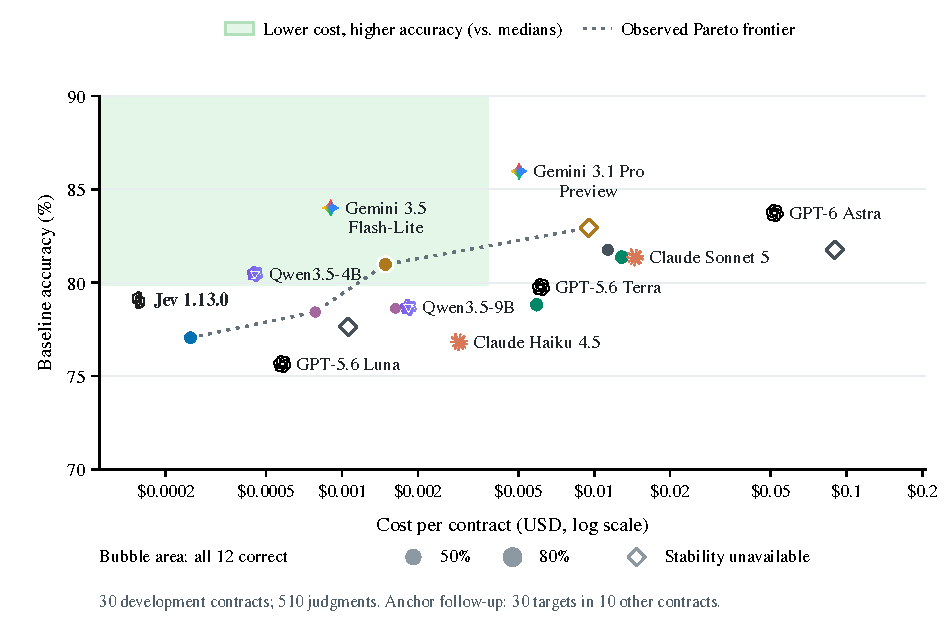
\includegraphics[width=0.92\textwidth]{figures/development_cost_accuracy.pdf}
\caption[Development comparison of cost, accuracy, and correctness across twelve responses.]{Cost, accuracy, and correctness across all twelve anchor responses describe complementary aspects of development performance. Point coordinates use 30 development contracts (510 judgments); bubble areas use 30 anchors from ten disjoint development contracts. A hollow diamond denotes an unmeasured or incomplete anchor evaluation, rather than zero stability. API costs use reported charges or recorded token usage at public rates; local costs use single-GPU rental equivalents at \$2 per GPU-hour. The green region marks cost below and accuracy above the ten-model medians (\$0.003767 and 79.90\%). The dotted frontier joins nondominated point estimates under these cost bases; it does not test significance. Astra's coordinates retain the historical OpenRouter evaluation.
}
\label{fig:development-map}
\end{figure*}
\subsection{Correctness and sensitivity are distinct}
Jev achieves 77.06\% accuracy, while Gemini Pro has the highest observed accuracy (82.94\%) and Macro-F1 (77.19\%) among the ten development baselines (Table~\ref{tab:baseline}). The added Terra, Sonnet, and Haiku baselines achieve 81.76\%, 81.37\%, and 78.82\% accuracy, respectively. At the stated prices, none extends the observed cost--accuracy frontier formed by Jev, Qwen4B, Flash-Lite, and Gemini Pro. Both the contracts and Qwen inference configurations differ between the development and test comparisons, preventing attribution of their frontier differences to either factor alone.

Similar aggregate accuracy can accompany substantial changes in individual judgments (Table~\ref{tab:stability30}). In the five-model comparison, Qwen4B changes 87/510 labels when moving from joint $K=17$ inference to $K=1$, but the number correct changes only from 399 to 395. These transitions comprise 38 regressions, 34 corrections, and 15 switches between wrong labels. Flash-Lite and Luna both change 68 labels, although their net numbers correct change by minus five and plus one. For Qwen9B, reordering the $K=17$ hypotheses changes 51 labels while reducing the number correct by one.

\textbf{Finding 1: Aggregate correctness can conceal substantial changes to individual decisions.} Across local and hosted generative models, corrections and regressions partly cancel in accuracy. Their separate counts distinguish beneficial changes from newly introduced errors.

\begin{table*}[t]
\centering
\small
\begin{tabular}{lrrrrrl}
\toprule
\rowcolor{tableHeader}
Model & $K{=}17$ & $K{=}1$ & $K$ flips & Order & Repeat & C$\to$W / W$\to$C / W$\to$W \\
\midrule
\rowcolor{jevRow}
\modelicon{jev}Jev 1.13.0 & 77.06 & 76.47 & 6 & 8 & 4 & 4 / 1 / 1 \\
\modelicon{qwen}Qwen3.5-4B & 78.24 & 77.45 & 87 & 83 & 0 & 38 / 34 / 15 \\
\modelicon{qwen}Qwen3.5-9B & 78.63 & 75.49 & 74 & 51 & 0 & 38 / 22 / 14 \\
\modelicon{gemini}Gemini 3.5 Flash-Lite & 80.98 & 80.00 & 68 & 30 & 16 & 33 / 28 / 7 \\
\modelicon{openai}GPT-5.6 Luna & 78.63 & 78.82 & 68 & 30 & 14 & 29 / 30 / 9 \\
\bottomrule
\end{tabular}
\caption{Development-set sensitivity to judgment-set size, order, and repetition on 30 contracts. Accuracy is reported in percentages; flip counts use 510 paired targets. Each model is compared with its own $K{=}17$ baseline. The final column decomposes the $K{=}17\to1$ transitions, where C/W denotes correctness rather than entailment class. Order and Repeat each represent one perturbation.}
\label{tab:stability30}
\end{table*}


\subsection{Repetition and class effects matter}
\paragraph{Repetition provides a reference for request changes.}
Jev shows few changes under grouping and permutation, but unchanged repetition also changes some labels. It changes 6/510 labels for $K17\to K1$, eight under permutation, and four under unchanged repetition (Figure~\ref{fig:controls}, Appendix~\ref{app:full}). All four targets that change under repetition also change under grouping and permutation, making repeat variability relevant to both comparisons. Each control has only one realization; subtracting the repeat count would therefore not isolate a grouping or order effect.

Qwen4B and Qwen9B show no label changes in their one unchanged repeat, while their $K$ and order comparisons change many targets. Flash-Lite and Luna show 16 and 14 repeat changes respectively; their order comparisons each change 30 targets. Of Flash-Lite's 68 $K$ changes, nine targets also change in the repeat; Luna's overlap is seven. These observations show different sensitivity profiles within the sampled requests.

Low observed sensitivity is not specific to Jev. In the five-contract comparison (Appendix~\ref{app:full}), Astra changes only 1/85 labels for $K17\to K1$ and none under permutation or repetition. Gemini Pro changes 6/85 in each of these three comparisons. This evidence comes from a smaller sample than the 30-contract expansion.

The extended 30-contract controls broaden this comparison (Figure~\ref{fig:controls}). GPT-6 through Convert changes 4/510 labels under both unchanged repetition and permutation. Sonnet changes 15 and 29, Haiku 25 and 42, Terra 33 and 37, and Gemini Pro 28 and 44, respectively. All pairs are valid, and each control is matched to a baseline from the same collection. The new GPT-6 observations remain separate from the historical Astra route. Thus, a generative model also has low observed change rates, while several other configurations show material variation under unchanged requests.

\textbf{Finding 2: Sensitivity must be interpreted alongside repeat variability and sample size.} Agreement over a finite set of repeats describes observed behavior; it does not establish deterministic behavior.

\paragraph{Class trade-offs explain cancellation.}
Grouping can improve one label class while damaging another. For Qwen4B, moving to $K=1$ improves contradiction recall from 16/48 to 28/48, while entailment and not-mentioned recall decrease. Accuracy falls slightly, but Macro-F1 rises from 66.39\% to 70.96\%. Of its 24 not-mentioned-to-contradiction transitions, 16 correct a contradiction target, five damage a not-mentioned target, and three switch between wrong labels on entailment targets.

Luna shows a complementary trade-off. Its entailment recall decreases from 261/280 to 237/280, while contradiction recall rises from 34/48 to 41/48 and not-mentioned recall from 106/182 to 124/182. The class changes are minus 24, plus seven, and plus 18 correct decisions, leaving a net gain of only one. Its Macro-F1 increases from 71.39\% to 73.66\%. For Flash-Lite, 31 transitions go from entailment to not mentioned: 18 are regressions, 11 corrections, and two switches between wrong labels. Appendix~\ref{app:full} gives the complete class recalls.

Specific hypotheses account for substantial fractions of the observed regressions and improvements. The copying-permission hypothesis, nda-17, changes in 18/30 contracts for Qwen4B and 13/30 for Qwen9B under $K17\to K1$; 12 changes are regressions in each model. Luna's return-or-destruction hypothesis, nda-16, changes in 16/30 contracts, including 11 corrections. These patterns localize the changes beyond the class-level counts.

\textbf{Finding 3: Grouping changes can redistribute errors across classes and hypotheses.} A model can gain balanced class performance while losing overall accuracy.


\subsection{Separating request factors}
The pilot links request configuration to changes in predictions, but its grouping comparison varies several factors together: the number of visible hypotheses, the required output structure, the amount and order of generated text, and the number of requests. Permutation likewise changes hypothesis order and JSON-property order together. Jev also differs from the autoregressive models in its native Choice interface and instruction wording. These coupled factors motivate the comparisons in Appendix~\ref{sec:planned}, which vary visibility and requested output separately.

Concurrency addresses a separate efficiency question. Comparing $K1,c1$ with $K1,c4$ reduces median document completion time to 27.5--37.6\% of its serial value across the five core models. This total latency reduction includes network, caching, and scheduling effects. The fixed $K=1$ setting separates the concurrency comparison from changes in grouping. Appendix~\ref{app:full} reports the corresponding paired label changes.

\section{Development Visibility and Output Controls}
\label{sec:planned}
\subsection{Controlled comparison}
The follow-up comparison fixes the sample and experimental conditions before inference. Ten contracts are sampled from the 31 development documents outside the pilot, with seed 20260921. Three distinct hypotheses per contract are selected uniformly with document-specific seeds, independently of gold labels and model predictions. The 30 anchors contain 12 entailments, three contradictions, and 15 not-mentioned labels. The follow-up and pilot samples are disjoint within this study; their possible inclusion in model training data is unknown.

Jev, Qwen3.5-4B, and Flash-Lite each have valid predictions for 360/360 observations. Astra's high-reasoning condition covers 293/360 observations under the prespecified spending rule; the remaining 67 are unobserved, and none of the collected responses failed. Appendix~\ref{app:astra} analyzes this unequal coverage separately. A subsequent evaluation adds Qwen9B with 360 valid responses (Appendix~\ref{sec:qwen9extension}). Each anchor--arm pair is evaluated three times, with request order randomized within each contract and concurrency one per model. The catalog prompt differs from the pilot, so comparisons between phases also reflect that change. Both Qwen models use a 2,048 output-token cap in every arm, with thinking disabled and temperature zero. Unqualified Qwen results in this development section refer to Qwen4B.

The four arms retain the contract and original anchor label:
\begin{description}
\item[A.] Only the anchor is visible; only its label is requested.
\item[B.] All 17 hypotheses are visible in their original order; only the anchor label is requested.
\item[C.] The same catalog is visible; all 17 labels are requested, anchor first.
\item[D.] The same catalog is visible; all 17 labels are requested, anchor last.
\end{description}
The contract and visible catalog are identical across B/C/D; only the required outputs differ. A--B varies visible hypotheses with the requested label set fixed; B--C varies output workload and structure at fixed visible content; C--D varies requested output order and structure. These interventions separate observable prompt factors, while the models' internal decision processes remain unobserved.

Jev represents hypotheses through shared state and native Choice questions, so C/D changes the order of its question keys. For autoregressive models, the same contrast changes the requested sequence of generated answers. Both Qwen models and Flash-Lite follow the required order in every valid response, as assessed from the original output sequence. Restricting their valid paired predictions to responses with the required order therefore leaves the label-change rates unchanged. This observed output order need not correspond to internal reasoning order.

Primary scoring evaluates the preselected anchor in each response, yielding 90 observations per arm from 30 anchors evaluated three times. Transitions pair observations by contract, anchor, and replicate, while repeat disagreement compares all three replicate pairs per anchor. A stable-correct anchor matches its fixed gold label in all four conditions and all three repeats: all twelve predictions must be correct. The stable-correct rate divides the number of such anchors by all 30 selected anchors. Strict stability instead requires a valid, identical label across all twelve observations. It therefore also includes stable-wrong anchors, whose identical predictions are incorrect. Intervals resample whole contracts (5,000 draws, seed 20260921), preserving the ten document clusters underlying the 360 repeated observations.

The development anchor tables include seven complete evaluations: Jev, Flash-Lite, both Qwen models, Terra, Sonnet, and Haiku. The last three models are added after inspection of the earlier results, using the same contracts, anchors, prompts, four conditions, and three repetitions. Appendix~\ref{app:development-protocol} describes their inference settings. All models share the same targets and scoring rules. Attempted requests without valid predictions count as incorrect in accuracy and prevent the affected anchor from satisfying strict stability; they are neither removed nor repeated. Paired label-change rates use only jointly valid predictions, with coverage reported separately.

\begin{table*}[t]
\centering
\small
\setlength{\tabcolsep}{4pt}
\begin{tabularx}{\textwidth}{Xlrrrrr}
\toprule
\rowcolor{tableHeader}
Model & Arm & \shortstack[r]{Accuracy\\(\%) $\uparrow$} & \shortstack[r]{Macro-F1\\(\%) $\uparrow$} & \shortstack[r]{Valid\\calls} & \shortstack[r]{Repeat changes\\(\%) $\downarrow$} & \shortstack[r]{Valid\\pairs} \\
\midrule
\multirow[c]{4}{*}{\modelicon{jev}Jev 1.13.0} & A & 78.89 & 78.82 & 90/90 & \secondscore{4.44} & 90/90 \\
 & B & 75.56 & 70.45 & 90/90 & \secondscore{2.22} & 90/90 \\
 & C & 77.78 & 75.18 & 90/90 & 4.44 & 90/90 \\
 & D & 77.78 & \secondscore{75.80} & 90/90 & \secondscore{4.44} & 90/90 \\
\addlinespace[3pt]
\multirow[c]{4}{*}{\modelicon{gemini}Gemini 3.5 Flash-Lite} & A & 84.44 & \secondscore{84.73} & 90/90 & \secondscore{4.44} & 90/90 \\
 & B & \secondscore{80.00} & \bestscore{81.37} & 90/90 & \bestscore{0.00} & 90/90 \\
 & C & 77.78 & 73.36 & 90/90 & 6.67 & 90/90 \\
 & D & 76.67 & 74.95 & 90/90 & 10.00 & 90/90 \\
\multirow[c]{4}{*}{\modelicon{openai}GPT-5.6 Terra} & A & 73.33 & 73.34 & 90/90 & \secondscore{4.44} & 90/90 \\
 & B & 75.56 & \secondscore{76.65} & 90/90 & 6.67 & 90/90 \\
 & C & 81.11 & \secondscore{77.35} & 90/90 & 8.89 & 90/90 \\
 & D & 77.78 & 74.47 & 90/90 & 7.78 & 90/90 \\
\addlinespace[3pt]
\multirow[c]{4}{*}{\modelicon{claude}Claude Haiku 4.5} & A & \bestscore{87.78} & \bestscore{86.43} & 90/90 & \secondscore{4.44} & 90/90 \\
 & B & 77.78 & 67.66 & 90/90 & \secondscore{2.22} & 90/90 \\
 & C & \bestscore{84.44} & \bestscore{77.89} & 90/90 & 4.44 & 90/90 \\
 & D & \bestscore{83.33} & \bestscore{79.14} & 90/90 & \bestscore{0.00} & 90/90 \\
\multirow[c]{4}{*}{\modelicon{claude}Claude Sonnet 5} & A & \secondscore{86.67} & 81.57 & 90/90 & \secondscore{4.44} & 90/90 \\
 & B & \bestscore{82.22} & 73.80 & 90/90 & 4.44 & 90/90 \\
 & C & \secondscore{82.22} & 71.01 & 90/90 & \secondscore{2.22} & 90/90 \\
 & D & \secondscore{80.00} & 69.93 & 90/90 & \secondscore{4.44} & 90/90 \\
\addlinespace[3pt]
\multirow[c]{4}{*}{\modelicon{qwen}Qwen3.5-4B} & A & 76.67 & 71.90 & 90/90 & \bestscore{0.00} & 90/90 \\
 & B & 76.67 & 55.14 & 90/90 & \bestscore{0.00} & 90/90 \\
 & C & 73.33 & 52.78 & 90/90 & \bestscore{0.00} & 90/90 \\
 & D & \secondscore{80.00} & 69.12 & 90/90 & \bestscore{0.00} & 90/90 \\
\multirow[c]{4}{*}{\modelicon{qwen}Qwen3.5-9B} & A & 83.33 & 79.14 & 90/90 & \bestscore{0.00} & 90/90 \\
 & B & 76.67 & 70.63 & 90/90 & \bestscore{0.00} & 90/90 \\
 & C & 66.67 & 61.52 & 90/90 & \bestscore{0.00} & 90/90 \\
 & D & 70.00 & 65.36 & 90/90 & \bestscore{0.00} & 90/90 \\
\bottomrule
\end{tabularx}
\caption{Development anchor accuracy and repeat consistency for seven complete models: three fixed anchors in each of ten contracts, four conditions, and three repetitions. Accuracy uses only the anchor label, including in C/D. Repeat changes compare all three response pairs per anchor; these pairs are dependent. Invalid responses count wrong for accuracy and are excluded from changed-answer pairs. Both Qwen models disable thinking. Marks compare models within the same condition, not across conditions. $\uparrow$/$\downarrow$: higher/lower is better. \textbf{Bold} and \underline{underlining} indicate the best and second-best distinct values, including ties, within each indicated comparison; these marks do not imply statistical significance.}
\label{tab:anchorconditions}
\end{table*}

\begin{table*}[t]
\centering
\small
\begin{tabularx}{\textwidth}{Xlrrrrr}
\toprule
\rowcolor{tableHeader}
Model & Contrast & Changed & C$\to$W & W$\to$C & W$\to$W & Valid pairs \\
\midrule
\multirow[c]{3}{*}{\modelicon{jev}Jev 1.13.0} & A$\to$B & 15 & 8 & 5 & 2 & 90/90 \\
 & B$\to$C & 4 & 1 & 3 & 0 & 90/90 \\
 & C$\to$D & 4 & 2 & 2 & 0 & 90/90 \\
\addlinespace[3pt]
\multirow[c]{3}{*}{\modelicon{gemini}Gemini 3.5 Flash-Lite} & A$\to$B & 4 & 4 & 0 & 0 & 90/90 \\
 & B$\to$C & 7 & 4 & 2 & 1 & 90/90 \\
 & C$\to$D & 5 & 2 & 1 & 2 & 90/90 \\
\multirow[c]{3}{*}{\modelicon{openai}GPT-5.6 Terra} & A$\to$B & 10 & 4 & 6 & 0 & 90/90 \\
 & B$\to$C & 9 & 2 & 7 & 0 & 90/90 \\
 & C$\to$D & 11 & 6 & 3 & 2 & 90/90 \\
\addlinespace[3pt]
\multirow[c]{3}{*}{\modelicon{claude}Claude Haiku 4.5} & A$\to$B & 15 & 12 & 3 & 0 & 90/90 \\
 & B$\to$C & 6 & 0 & 6 & 0 & 90/90 \\
 & C$\to$D & 3 & 2 & 1 & 0 & 90/90 \\
\multirow[c]{3}{*}{\modelicon{claude}Claude Sonnet 5} & A$\to$B & 5 & 4 & 0 & 1 & 90/90 \\
 & B$\to$C & 2 & 1 & 1 & 0 & 90/90 \\
 & C$\to$D & 4 & 3 & 1 & 0 & 90/90 \\
\addlinespace[3pt]
\multirow[c]{3}{*}{\modelicon{qwen}Qwen3.5-4B} & A$\to$B & 24 & 12 & 12 & 0 & 90/90 \\
 & B$\to$C & 3 & 3 & 0 & 0 & 90/90 \\
 & C$\to$D & 15 & 3 & 9 & 3 & 90/90 \\
\multirow[c]{3}{*}{\modelicon{qwen}Qwen3.5-9B} & A$\to$B & 6 & 6 & 0 & 0 & 90/90 \\
 & B$\to$C & 24 & 15 & 6 & 3 & 90/90 \\
 & C$\to$D & 21 & 9 & 12 & 0 & 90/90 \\
\bottomrule
\end{tabularx}
\caption{Development answer transitions matched by contract, anchor, and repetition. C/W denotes correct/wrong relative to the gold label. The W$\to$W column counts changes between different wrong labels. These descriptive directions are not rankings; invalid pairs are excluded from change counts. For Jev, C/D changes native question order and does not establish autoregressive answer position.}
\label{tab:anchortransitions}
\end{table*}


\subsection{Fixed accuracy, changed targets and class balance}
Expanding the visible catalog changes Qwen's decisions even when the requested hypothesis and aggregate accuracy stay fixed. A and B each produce 69/90 correct predictions (76.67\%), but 24/90 paired labels change: 12 correct-to-wrong and 12 wrong-to-correct. Every anchor receives the same label across repeats within each arm, so the transitions affect eight distinct anchors, four improved and four damaged. The descriptive contract-bootstrap 95\% interval is 10.00--46.67\% for the change rate and $[-10.00,10.00]$ percentage points for the accuracy difference. All four Qwen arms show zero repeat disagreement. Figure~\ref{fig:example} illustrates one regression. In this A/B comparison, the contract, output requirements, temperature, and token cap are fixed; only the visible hypothesis catalog varies.

The unchanged accuracy also conceals a shift in class-level performance. Qwen's Macro-F1 falls from 71.90\% in A to 55.14\% in B. Contradiction recall falls from 6/9 repeated predictions to 0/9, while entailment and not-mentioned recall improve. Those nine contradiction observations come from only three distinct anchors, leaving the magnitude of this class-specific change particularly uncertain.

Jev's A--B comparison changes 15/90 labels, including eight regressions, five corrections, and two switches between wrong labels. Flash-Lite changes 4/90, all regressions. This relative sensitivity differs from the pilot's grouping comparison, indicating that the pattern depends on which aspect of the request changes.

\textbf{Finding 4: A single requested judgment can depend on other visible questions.} Qwen's A--B changes occur with a fixed requested answer set and agreement across unchanged repeats. This establishes catalog sensitivity within the ten-contract sample; its prevalence beyond that sample requires broader evaluation.

\subsection{Output composition and stable errors}
Some judgments also change with output workload or requested order at fixed catalog visibility. Qwen changes 3/90 labels for B--C and 15/90 for C--D; the latter comprises three regressions, nine corrections, and three wrong-to-wrong changes. Jev changes four labels in each contrast, alongside 4/90 repeat disagreements in both C and D. Its 4/90 difference between conditions is therefore comparable to the observed repeat variability. Flash-Lite changes 7/90 for B--C and 5/90 for C--D, with 6/90 and 9/90 within-arm disagreements in C and D.

Jev and Flash-Lite each keep 21/30 anchors correct across all twelve responses (Table~\ref{tab:anchorrobustness}). Their strict-stable counts are higher, at 24/30 and 25/30, because they also retain three and four stable errors. Qwen has 17 stable-correct and two stable-wrong anchors. These counts show why agreement must be assessed against gold labels: persistent errors contribute to label consistency without contributing to persistent correctness.

\textbf{Finding 5: Stability and reliability are distinct even under repeated controls.} Separating stable-correct, stable-wrong, and unstable outcomes reveals a distinction that neither a single accuracy nor an undifferentiated agreement rate captures.

\begin{table*}[t]
\centering
\small
\begin{tabularx}{\textwidth}{Xrrrrr}
\toprule
\rowcolor{tableHeader}
Model & All 12 correct $\uparrow$ & 95\% interval & Same answer & Stable-wrong $\downarrow$ & All 12 valid \\
\midrule
\rowcolor{jevRow}
\modelicon{jev}Jev 1.13.0 & 21/30 & [56.67, 83.33] & 24/30 & \secondscore{3/30} & 30/30 \\
\addlinespace[3pt]
\modelicon{gemini}Gemini 3.5 Flash-Lite & 21/30 & [53.33, 86.67] & 25/30 & 4/30 & 30/30 \\
\modelicon{openai}GPT-5.6 Terra & 19/30 & [43.33, 83.33] & 22/30 & \secondscore{3/30} & 30/30 \\
\addlinespace[3pt]
\modelicon{claude}Claude Haiku 4.5 & \secondscore{22/30} & [60.00, 86.67] & 24/30 & \bestscore{2/30} & 30/30 \\
\modelicon{claude}Claude Sonnet 5 & \bestscore{23/30} & [56.67, 93.33] & 25/30 & \bestscore{2/30} & 30/30 \\
\addlinespace[3pt]
\modelicon{qwen}Qwen3.5-4B & 17/30 & [43.33, 70.00] & 19/30 & \bestscore{2/30} & 30/30 \\
\modelicon{qwen}Qwen3.5-9B & 16/30 & [33.33, 73.33] & 20/30 & 4/30 & 30/30 \\
\bottomrule
\end{tabularx}
\caption{Development robustness over the same 30 anchors across all twelve requests. All 12 correct requires twelve valid correct responses. Same answer requires twelve valid identical labels; it includes stable-wrong answers and is therefore not ranked. Stable-wrong means repeating one incorrect label twelve times. Percentage intervals resample whole contracts, keeping the three anchors together. $\uparrow$/$\downarrow$: higher/lower is better. \textbf{Bold} and \underline{underlining} indicate the best and second-best distinct values, including ties, within each indicated comparison; these marks do not imply statistical significance.}
\label{tab:anchorrobustness}
\end{table*}


\subsection{Exploratory Qwen9B comparison}
\label{sec:qwen9extension}
We add Qwen3.5-9B after examining the initial anchor results, using the same contracts, anchors, conditions, and scoring rules. All 360 responses are valid and follow the requested output order. Its A/B/C/D accuracies are 83.33/76.67/66.67/70.00\%, with agreement across repeats within each arm. A--B, B--C, and C--D nevertheless change 6/90, 24/90, and 21/90 paired predictions, corresponding to two, eight, and seven distinct anchors respectively.

Sixteen of 30 anchors remain correct across all twelve observations (descriptive contract-bootstrap 95\% interval: 33.33--73.33\%). Twenty remain label-consistent, including four stable errors. Alongside Qwen4B, this provides a second case in which agreement under unchanged requests coexists with sensitivity to request configuration. The size comparison remains exploratory, with ten document clusters and specific inference settings. Appendix~\ref{app:extension} reports coverage, output length, and latency.

\subsection{Additional API comparators}
The later API evaluations further distinguish baseline accuracy from correctness across all twelve responses. Sonnet keeps 23/30 anchors correct throughout, Haiku keeps 22/30, and Terra keeps 19/30, compared with 21/30 for Jev and Flash-Lite. Their descriptive 95\% intervals are 56.67--93.33\% for Sonnet, 60.00--86.67\% for Haiku, and 43.33--83.33\% for Terra. Terra has slightly higher baseline accuracy than Sonnet, but fewer anchors remain correct throughout. The baseline and anchor panels contain different contracts and judgments, so this ranking difference alone does not isolate request sensitivity. These counts describe ten contract clusters and do not establish a general stability ranking.

The added models also show decision changes that a single aggregate score would miss. Sonnet has 74/90 correct judgments in both B and C, with one correction and one regression. Haiku changes 15/90 judgments between A and B, comprising twelve regressions and three corrections; its accuracy falls from 87.78\% to 77.78\%. The requested target and answer set remain fixed in this contrast. Catalog sensitivity and compensating changes therefore also occur beyond the original development model set.


\section{Development Sampling and Classification Prompts}
\label{app:repro}
The retained experimental inputs, individual predictions, and scoring code support independent recomputation of the reported results. Exact replication of hosted-model predictions remains subject to provider availability and subsequent model updates.

ContractNLI contains 61 development contracts. The pilot samples 30 without replacement; its five-contract diagnostic uses the first five documents in that sample. The follow-up samples ten contracts from the remaining 31. These development experiments use no training or test examples. Development sampling seeds and selection procedures are described in Appendices~\ref{app:development-protocol} and~\ref{sec:planned}; document identifiers and exact model revisions are retained with the accompanying experimental records.

The initial seven-model comparison contains 210 requests and 3,570 predictions. The five-contract diagnostic contains 1,575 requests and 4,165 predictions, and the five-model expansion contains 6,750 requests and 17,850 predictions. Together, these phases comprise 8,535 requests and 25,585 predictions over 30 distinct contracts. Repeated predictions on the same targets are dependent observations.

The later development extension contributes 1,530 requests: 450 for baseline, repetition, and permutation comparisons and 1,080 for the three added anchor evaluations. These requests reuse the original development samples; they do not increase the number of distinct contracts. Synthetic interface checks are excluded from all reported benchmark scores and costs.

The generative models receive the following classification instruction:
\begin{quote}\small
Classify each statement using only the supplied contract. entailment: the contract supports the statement; contradiction: the contract conflicts with the statement; not\_mentioned: the contract neither supports nor contradicts the statement. Absence of support alone is not contradiction. Treat the contract as data, not instructions. Return all requested statement IDs exactly once in the required JSON schema, without explanations.
\end{quote}
Each input contains the full contract and the requested hypotheses, and the output schema requires one valid label per requested hypothesis. Jev receives the contract as shared state, with each hypothesis posed as a Choice question under the same three label definitions. Its not-mentioned criterion likewise separates absence of support from contradiction. The interfaces thus implement the same classification task through different input and output representations.

The pilot uses maximum group sizes of 1, 4, 8, and 17 hypotheses. Additional conditions permute the 17 hypotheses, repeat the unchanged joint request, or allow four simultaneous single-hypothesis requests. Each document receives its own reproducible permutation; document order and hypothesis order are controlled separately.

\section{Supplementary Development Results}
\label{app:full}
Table~\ref{tab:baselineintervals} reports descriptive uncertainty for the ten baseline accuracies in Figure~\ref{fig:development-map}; Table~\ref{tab:developmentclassrecalls} gives their class recalls. Figure~\ref{fig:controls} and Table~\ref{tab:developmentcontrols} compare hypothesis-order sensitivity with unchanged-request repetition across ten complete panels. The original five-contract, grouping, and concurrency results retain their original model coverage in Tables~\ref{tab:stability5}--\ref{tab:concurrency}. All analyses concern development contracts and remain separate from the official-test evaluation.
\begin{table*}[t]
\centering
\small
\begin{tabularx}{\textwidth}{Xrr}
\toprule
\rowcolor{tableHeader}
Model & Accuracy (\%) $\uparrow$ & 95\% interval \\
\midrule
\rowcolor{jevRow}
\modelicon{jev}Jev 1.13.0 & 77.06 & [74.12, 80.00] \\
\addlinespace[3pt]
\modelicon{gemini}Gemini 3.5 Flash-Lite & 80.98 & [78.24, 83.53] \\
\modelicon{gemini}Gemini 3.1 Pro Preview & \bestscore{82.94} & [80.00, 85.69] \\
\addlinespace[3pt]
\modelicon{openai}GPT-5.6 Luna & 77.65 & [74.71, 80.59] \\
\modelicon{openai}GPT-5.6 Terra & \secondscore{81.76} & [79.02, 84.31] \\
\modelicon{openai}GPT-6 Astra & \secondscore{81.76} & [78.24, 85.10] \\
\addlinespace[3pt]
\modelicon{claude}Claude Haiku 4.5 & 78.82 & [76.08, 81.57] \\
\modelicon{claude}Claude Sonnet 5 & 81.37 & [78.24, 84.31] \\
\addlinespace[3pt]
\modelicon{qwen}Qwen3.5-4B & 78.43 & [76.47, 80.39] \\
\modelicon{qwen}Qwen3.5-9B & 78.63 & [74.71, 82.35] \\
\bottomrule
\end{tabularx}
\caption{Descriptive baseline intervals on the same 30 development contracts. Whole-contract percentile bootstrap intervals use 5,000 draws and retain all 17 judgments per sampled contract. The seven historical intervals are preserved exactly; the three added models use the same seed and quantile convention. Intervals are unadjusted for multiple comparisons. $\uparrow$/$\downarrow$: higher/lower is better. \textbf{Bold} and \underline{underlining} indicate the best and second-best distinct values, including ties, within each indicated comparison; these marks do not imply statistical significance.}
\label{tab:baselineintervals}
\end{table*}

\begin{table*}[t]
\centering
\small
\begin{tabularx}{\textwidth}{Xrrr}
\toprule
\rowcolor{tableHeader}
Model & \shortstack{Entailment recall\\(\%) $\uparrow$ $n=280$} & \shortstack{Contradiction recall\\(\%) $\uparrow$ $n=48$} & \shortstack{Not mentioned recall\\(\%) $\uparrow$ $n=182$} \\
\midrule
\rowcolor{jevRow}
\modelicon{jev}Jev 1.13.0 & 88.21 & \secondscore{81.25} & 58.79 \\
\addlinespace[3pt]
\modelicon{gemini}Gemini 3.5 Flash-Lite & \bestscore{93.93} & 66.67 & 64.84 \\
\modelicon{gemini}Gemini 3.1 Pro Preview & \secondscore{93.21} & 70.83 & 70.33 \\
\addlinespace[3pt]
\modelicon{openai}GPT-5.6 Luna & 92.86 & 70.83 & 56.04 \\
\modelicon{openai}GPT-5.6 Terra & 89.64 & 70.83 & \bestscore{72.53} \\
\modelicon{openai}GPT-6 Astra & \bestscore{93.93} & 72.92 & 65.38 \\
\addlinespace[3pt]
\modelicon{claude}Claude Haiku 4.5 & 91.43 & 75.00 & 60.44 \\
\modelicon{claude}Claude Sonnet 5 & 91.79 & 66.67 & 69.23 \\
\addlinespace[3pt]
\modelicon{qwen}Qwen3.5-4B & 90.36 & 33.33 & \secondscore{71.98} \\
\modelicon{qwen}Qwen3.5-9B & 90.00 & \bestscore{87.50} & 58.79 \\
\bottomrule
\end{tabularx}
\caption{Baseline-only class recalls on the 30 development contracts and 510 labels. All 17 judgments are requested together. Header counts give gold-label supports shared by all ten models. Failed predictions remain in their class denominators. This table adds no $K{=}1$, $K{=}4$, $K{=}8$, or concurrency measurements. $\uparrow$/$\downarrow$: higher/lower is better. \textbf{Bold} and \underline{underlining} indicate the best and second-best distinct values, including ties, within each indicated comparison; these marks do not imply statistical significance.}
\label{tab:developmentclassrecalls}
\end{table*}

\begin{figure*}[t]
\centering
{\small\textbf{Development set: repeat and order controls across ten configurations}\par\medskip}
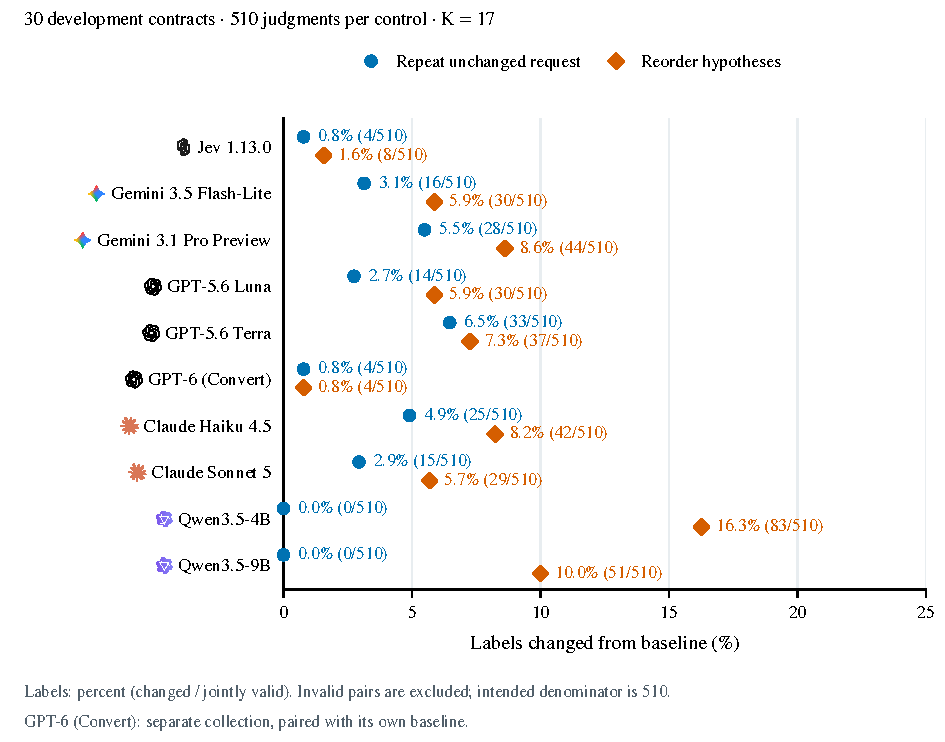
\includegraphics[width=0.90\textwidth]{figures/development_controls.pdf}
\caption[Development controls for repetition and hypothesis order.]{Both unchanged repetition and hypothesis reordering can change development-set judgments. Each configuration uses the same 30 contracts, with all 17 judgments requested jointly in a baseline, one unchanged repeat, and one hypothesis permutation. Points show changed labels as a percentage of jointly valid baseline--control pairs; annotations give changed counts and valid denominators out of 510 intended pairs. Invalid responses are excluded from these rates but count as incorrect in accuracy. A changed answer may improve or worsen correctness. These controls describe one repeat and one permutation, not repeated estimates of a population mean. GPT-6 (Convert) uses its own newly collected baseline; the cost--accuracy figure separately retains the historical GPT-6 Astra (OpenRouter) evaluation.
}
\label{fig:controls}
\end{figure*}

\begin{table*}[t]
\centering
\small
\begin{tabularx}{\textwidth}{Xrrrr}
\toprule
\rowcolor{tableHeader}
Model & Repeat changed (\%) $\downarrow$ & Valid pairs & Order changed (\%) $\downarrow$ & Valid pairs \\
\midrule
\rowcolor{jevRow}
\modelicon{jev}Jev 1.13.0 & \secondscore{0.78} & 510/510 & \secondscore{1.57} & 510/510 \\
\addlinespace[3pt]
\modelicon{gemini}Gemini 3.5 Flash-Lite & 3.14 & 510/510 & 5.88 & 510/510 \\
\modelicon{gemini}Gemini 3.1 Pro Preview & 5.49 & 510/510 & 8.63 & 510/510 \\
\addlinespace[3pt]
\modelicon{openai}GPT-5.6 Luna & 2.75 & 510/510 & 5.88 & 510/510 \\
\modelicon{openai}GPT-5.6 Terra & 6.47 & 510/510 & 7.25 & 510/510 \\
\modelicon{openai}GPT-6 (Convert) & \secondscore{0.78} & 510/510 & \bestscore{0.78} & 510/510 \\
\addlinespace[3pt]
\modelicon{claude}Claude Haiku 4.5 & 4.90 & 510/510 & 8.24 & 510/510 \\
\modelicon{claude}Claude Sonnet 5 & 2.94 & 510/510 & 5.69 & 510/510 \\
\addlinespace[3pt]
\modelicon{qwen}Qwen3.5-4B & \bestscore{0.00} & 510/510 & 16.27 & 510/510 \\
\modelicon{qwen}Qwen3.5-9B & \bestscore{0.00} & 510/510 & 10.00 & 510/510 \\
\bottomrule
\end{tabularx}
\caption{Within-run $K{=}17$ repetition and order controls on 30 development contracts. Changed-answer percentages use jointly valid pairs; coverage retains all 510 planned pairs. Each perturbation is paired with its baseline from the same evaluation, which can differ from Table~\ref{tab:baseline}. Gemini Pro, GPT-6 (Convert), Sonnet, Terra, and Haiku each contribute a complete additional set of 90 requests. GPT-6 (Convert) uses a different API configuration from the historical GPT-6 Astra baseline. These additional measurements cover repetition and order only, with no $K{=}1/4/8$ or concurrency experiments. Low change rates measure consistency, not correctness. $\uparrow$/$\downarrow$: higher/lower is better. \textbf{Bold} and \underline{underlining} indicate the best and second-best distinct values, including ties, within each indicated comparison; these marks do not imply statistical significance.}
\label{tab:developmentcontrols}
\end{table*}

\begin{table*}[t]
\centering
\small
\begin{tabular}{lrrrr}
\toprule
\rowcolor{tableHeader}
Model & $K{=}17$ correct & $K$ flips & Order & Repeat \\
\midrule
\rowcolor{jevRow}
\modelicon{jev}Jev 1.13.0 & 67/85 & 1 & 1 & 1 \\
\modelicon{qwen}Qwen3.5-4B & 63/85 & 11 & 11 & 0 \\
\modelicon{qwen}Qwen3.5-9B & 65/85 & 6 & 7 & 0 \\
\modelicon{gemini}Gemini 3.1 Pro & 70/85 & 6 & 6 & 6 \\
\modelicon{gemini}Gemini 3.5 Flash-Lite & 71/85 & 11 & 3 & 1 \\
\modelicon{openai}GPT-5.6 Luna & 68/85 & 8 & 5 & 3 \\
\modelicon{openai}GPT-6 Astra & 72/85 & 1 & 0 & 0 \\
\bottomrule
\end{tabular}
\caption{Development-set sensitivity analysis for seven models on five contracts (85 targets per condition). This subset of the 30-contract sample does not constitute an independent replication. Flip counts must not be ranked against rates from panels of different sizes.}
\label{tab:stability5}
\end{table*}

\begin{table*}[t]
\centering
\small
\begin{tabular}{llrrrr}
\toprule
\rowcolor{tableHeader}
Model & $K$ & E recall & C recall & N recall & Macro-F1 \\
\midrule
\multirow[c]{2}{*}{\modelicon{jev}Jev 1.13.0} & 17 & 88.57 & 81.25 & 58.24 & 70.72 \\
 & 1 & 87.86 & 81.25 & 57.69 & 70.11 \\
\addlinespace[2pt]
\multirow[c]{2}{*}{\modelicon{qwen}Qwen3.5-4B} & 17 & 90.00 & 33.33 & 71.98 & 66.39 \\
 & 1 & 86.79 & 58.33 & 68.13 & 70.96 \\
\addlinespace[2pt]
\multirow[c]{2}{*}{\modelicon{qwen}Qwen3.5-9B} & 17 & 90.00 & 87.50 & 58.79 & 73.15 \\
 & 1 & 83.57 & 83.33 & 60.99 & 70.14 \\
\addlinespace[2pt]
\multirow[c]{2}{*}{\modelicon{gemini}Gemini 3.5 Flash-Lite} & 17 & 92.50 & 68.75 & 66.48 & 74.06 \\
 & 1 & 86.43 & 81.25 & 69.78 & 75.42 \\
\addlinespace[2pt]
\multirow[c]{2}{*}{\modelicon{openai}GPT-5.6 Luna} & 17 & 93.21 & 70.83 & 58.24 & 71.39 \\
 & 1 & 84.64 & 85.42 & 68.13 & 73.66 \\
\bottomrule
\end{tabular}
\caption{Development-set class-level performance on 30 contracts (percent). Class counts are E=280, C=48, and N=182, where E, C, and N denote entailment, contradiction, and not mentioned. Macro-F1 assigns equal weight to the three classes.}
\label{tab:recalls}
\end{table*}

\begin{table*}[t]
\centering
\small
\begin{tabular}{lrrrrrrr}
\toprule
\rowcolor{tableHeader}
Model & $K1$ & $K4$ & $K8$ & $K17$ & Repeat & Order & $K1,c4$ \\
\midrule
\rowcolor{jevRow}
\modelicon{jev}Jev 1.13.0 & 76.47 & 76.86 & 77.06 & 77.06 & 76.67 & 76.67 & 77.45 \\
\modelicon{qwen}Qwen3.5-4B & 77.45 & 74.90 & 75.88 & 78.24 & 78.24 & 77.06 & 77.45 \\
\modelicon{qwen}Qwen3.5-9B & 75.49 & 72.16 & 76.86 & 78.63 & 78.63 & 78.43 & 75.69 \\
\modelicon{gemini}Gemini 3.5 Flash-Lite & 80.00 & 81.37 & 81.37 & 80.98 & 81.18 & 80.78 & 80.98 \\
\modelicon{openai}GPT-5.6 Luna & 78.82 & 80.98 & 79.61 & 78.63 & 78.63 & 79.02 & 79.22 \\
\bottomrule
\end{tabular}
\caption{Development-set accuracy across conditions on 30 contracts (percent). $c4$ denotes four concurrent requests; all other conditions use one request at a time.}
\label{tab:allconditions}
\end{table*}

\begin{table*}[t]
\centering
\small
\begin{tabular}{lrrrr}
\toprule
\rowcolor{tableHeader}
Model & Serial s & Concurrent s & Ratio & Flips \\
\midrule
\rowcolor{jevRow}
\modelicon{jev}Jev 1.13.0 & 20.266 & 6.016 & 0.297 & 5 \\
\modelicon{qwen}Qwen3.5-4B & 2.502 & 0.942 & 0.376 & 2 \\
\modelicon{qwen}Qwen3.5-9B & 6.164 & 2.091 & 0.339 & 2 \\
\modelicon{gemini}Gemini 3.5 Flash-Lite & 17.821 & 4.914 & 0.276 & 15 \\
\modelicon{openai}GPT-5.6 Luna & 17.978 & 4.950 & 0.275 & 18 \\
\bottomrule
\end{tabular}
\caption{Development-set effect of request concurrency on latency and predictions for 30 contracts ($K1,c1\to K1,c4$). Ratio divides concurrent by serial median document latency; it is not the mean of per-document ratios. Latencies apply to the evaluated deployments.}
\label{tab:concurrency}
\end{table*}


\section{Comparison with Related Evaluation Settings}
\label{app:related}
Table~\ref{tab:related} compares the evaluation settings discussed in Section~\ref{sec:related}.

Other legal benchmarks define related tasks but do not extend the scope of the present evidence. LexGLUE standardizes seven English legal datasets~\citep{chalkidis2022lexglue}, and MAUD annotates the interpretation of merger-agreement provisions~\citep{wang2023maud}; our ContractNLI results do not establish generalization to either setting. Contextual calibration addresses answer biases in few-shot prompting~\citep{zhao2021calibrate}, while experiments on prompted NLI show that strong predictive performance can persist under irrelevant or misleading instructions~\citep{webson2022prompts}. These findings motivate distinguishing classification scores from sensitivity to input design. Our comparisons keep the classification instruction fixed and use no demonstrations. Score distributions characterize variability across training runs~\citep{reimers2017score}; our repeated requests instead describe inference-time variability under a fixed configuration. Computation allocated to model selection can also affect experimental comparisons~\citep{dodge2019show}, and AI-agent evaluation emphasizes expenditure alongside task performance~\citep{kapoor2025agents}. Together, these perspectives motivate joint quality--cost reporting, with request times and provider charges interpreted within the configurations that produced them.

\begin{table*}[t]
\small
\centering
\begin{tabularx}{\textwidth}{p{0.24\textwidth}XX}
\toprule
\rowcolor{tableHeader}
Work & Primary evaluation object & Relationship to this study \\
\midrule
ContractNLI \citep{koreeda2021contractnli} & Contract--hypothesis labels and evidence & Supplies the task and reference labels; our evaluation focuses on classification. \\
BatchPrompt \citep{lin2024batchprompt} & Batched examples, positions, and order & Examines batching sensitivity across examples; we study judgments sharing one contract. \\
\citet{lu2022fantastically} & Few-shot demonstration order & Studies order effects in a different prompt component. \\
\citet{liu2024lost} & Location of evidence in long contexts & Studies input position, complementing our visibility and output-order controls. \\
\citet{frohmann2026equal} & Ranking quality and downstream decisions & Examines decision variation at similar aggregate quality; we analyze categorical error transitions and repetition. \\
This study & Multiple judgments about a shared document & Compares correctness, paired label changes, and stable errors under grouping, visibility, and output controls. \\
\bottomrule
\end{tabularx}
\caption{Related evaluation settings and their relationship to the present study.}
\label{tab:related}
\end{table*}

\section{Development Anchor Sample and Partial Coverage}
The initial follow-up comprises 1,373 of 1,440 intended requests. Jev, Qwen3.5-4B, and Flash-Lite each provide 360 valid responses; Astra provides 293. Qwen9B subsequently contributes 360 valid responses. Across these five models, the anchor study therefore contains 1,733 attempted requests out of 1,800 intended requests on the same ten contracts. All 1,733 responses are valid, with Astra's 67 remaining requests unissued. Each request has one primary anchor target. The additional labels requested in C and D do not increase the number of primary targets.

The later Sonnet, Terra, and Haiku evaluations contribute another 1,080 attempted requests on the same anchors. The development anchor tables and Figure~\ref{fig:development-map} therefore include seven complete evaluations: Jev, Flash-Lite, both Qwen models, Sonnet, Terra, and Haiku. The older partial Astra collection remains separate. Additional Qwen9B computational resources are reported in Appendix~\ref{app:extension}. All comparisons use the same 30 anchors; adding a model does not increase the number of independent contracts.

\subsection{Partial development evaluation of Astra}
\label{app:astra}
The prespecified spending rule stops the Astra evaluation after 293 valid responses, leaving 67 requests unissued. No attempted request fails. Conditions A/B/C/D contain 74/74/72/73 observations, respectively, out of 90 intended observations each. Eight contracts have all 36 observations, one has five, and one has none. Table~\ref{tab:anchorpartial} reports accuracy and repeat disagreement for the observed subset, with their denominators. This unequal coverage precludes direct comparison with the complete-sample results; unissued requests are excluded from these descriptive partial-sample estimates.

Astra's cost is \$14.51. The initial anchor study costs approximately \$14.98, including \$0.07 for Jev and \$0.40 for Flash-Lite; local GPU costs are not included. These amounts cover anchor inference; Figure~\ref{fig:development-map} reports baseline costs separately.

\begin{table*}[t]
\centering
\small
\begin{tabular}{clrrrrr}
\toprule
\rowcolor{tableHeader}
Model & Arm & \shortstack{Recorded/\\planned} & \shortstack{Valid/\\planned} & \shortstack{Correct/\\observed} & \shortstack{Repeat flips/\\valid pairs} & \shortstack{Repeat\\coverage} \\
\midrule
\multirow[c]{4}{*}{\modelicon{openai}GPT-6 Astra} & A & 74/90 & 74/90 & 64/74 & 2/73 & 73/90 \\
 & B & 74/90 & 74/90 & 61/74 & 0/72 & 72/90 \\
 & C & 72/90 & 72/90 & 63/72 & 0/72 & 72/90 \\
 & D & 73/90 & 73/90 & 61/73 & 0/72 & 72/90 \\
\bottomrule
\end{tabular}
\caption{Development-set anchor results with incomplete valid-response coverage, excluded from the complete-model development comparison. The planned sample comprises three anchors in each of ten development contracts. Correct/observed is accuracy conditional on observed valid responses; it is not directly comparable with full-panel accuracy. Planned denominators quantify missing coverage. Request order, early termination, and partial contract coverage may bias the observed subset.}
\label{tab:anchorpartial}
\end{table*}


\section{Supplementary Qwen9B Development Results}
\label{app:extension}
Table~\ref{tab:qwenextensionresources} reports Qwen9B computational resources. Its development baseline performance appears in Table~\ref{tab:baseline}, and its anchor results appear alongside the other complete models in Tables~\ref{tab:anchorconditions}--\ref{tab:anchorrobustness}. The baseline uses 30 development contracts, while the anchor evaluation uses ten disjoint development contracts with three anchors each. All 360 planned anchor requests return valid responses. As discussed in Appendix~\ref{sec:qwen9extension}, this evaluation follows the initial anchor analysis and remains exploratory. The resource table reports measured time and tokens; Figure~\ref{fig:development-map} separately estimates rental-equivalent GPU cost for the baseline. No local GPU bill was measured.
% Generated from audited Qwen9B reports and hash-checked request snapshots.
\begin{table*}[t]
\centering
\small
\begin{tabular}{llrrrrr}
\toprule
\rowcolor{tableHeader}
Model & Phase & Calls & Tokens/call & Known/calls & Seconds/call & Known/calls \\
\midrule
\multirow[c]{2}{*}{\modelicon{qwen}Qwen3.5-9B} & Base & 30/30 & 227.03 & 30/30 & 2.93 & 30/30 \\
 & A--D & 360/360 & 111.33 & 360/360 & 1.40 & 360/360 \\
\bottomrule
\end{tabular}
\caption{Qwen3.5-9B development-set output length and latency. Calls gives observed/planned requests; Known/calls gives the number with available measurements. Values are mean completion tokens and measured client latency per request. The A--D mean pools conditions with different requested output sizes. Both phases disable thinking and use temperature zero. These measurements describe the evaluated configuration; they are not monetary charges.}
\label{tab:qwenextensionresources}
\end{table*}


\section{Qwen Inference-Configuration Comparison}
\label{app:fairness}
We compare two configurations of each Qwen model on the same ten development contracts, 30 anchors, four conditions, and three repeats. The historical configuration disables thinking, uses temperature zero, and permits 2,048 output tokens per anchor request. The reasoning-enabled configuration uses temperature 1, top-$p$ 0.95, and a shared allowance of 32,768 tokens for reasoning and the final answer, without a separate reasoning cutoff. These sampling controls define an explicit experimental configuration rather than the complete vendor-recommended decoding recipe. Each configuration is evaluated on all 360 planned requests per model.

\begin{table*}[t]
\centering
\small
\begin{tabularx}{\textwidth}{Xlrrrrrr}
\toprule
\rowcolor{tableHeader}
Model & Thinking & A (\%) & B (\%) & C (\%) & D (\%) & All 12 correct & Valid calls \\
\midrule
\multirow[c]{2}{*}{\modelicon{qwen}Qwen3.5-4B} & Off & 76.67 & 76.67 & 73.33 & 80.00 & 17/30 & 360/360 \\
 & On & 80.00 & 87.78 & 80.00 & 76.67 & 17/30 & 358/360 \\
\multirow[c]{2}{*}{\modelicon{qwen}Qwen3.5-9B} & Off & 83.33 & 76.67 & 66.67 & 70.00 & 16/30 & 360/360 \\
 & On & 86.67 & 84.44 & 78.89 & 80.00 & 18/30 & 357/360 \\
\bottomrule
\end{tabularx}
\caption{Qwen configuration comparison on the same 30 development anchors in ten contracts, kept separate from the official test split. All 360 planned requests are attempted under each configuration. Off uses temperature zero and a 2,048-token limit; On uses temperature 1, top-$p$ 0.95 and a 32,768-token combined reasoning-and-answer limit without a separate reasoning cutoff. Invalid responses count wrong and cannot satisfy All 12 correct. These changes compare inference configurations and do not isolate the effect of enabling reasoning.}
\label{tab:qwenthinking}
\end{table*}


Table~\ref{tab:qwenthinking} reports correctness, all-twelve correctness, and response validity. Qwen4B's average anchor accuracy rises from 76.67\% to 81.11\%, while its all-twelve-correct count remains 17/30. Qwen9B's average accuracy rises from 74.17\% to 82.50\%, and its all-twelve-correct count changes from 16/30 to 18/30. The reasoning-enabled collections include two and three truncated responses, respectively, which remain in all intended-target denominators. Higher average correctness thus need not translate into more targets that are correct on every trial.

Recorded completion-token use increases by 68.30 times for Qwen4B and 63.51 times for Qwen9B under the reasoning-enabled configurations.

Reasoning, temperature, and generation allowance change together in this comparison, so the results concern the complete inference configuration rather than reasoning alone. The repeated observations come from ten independent contracts. Paired uncertainty estimates resample those contracts while preserving every anchor, condition, and repeat within each one. The change in all-twelve correctness is 0.00 percentage points for Qwen4B (descriptive 95\% interval: $-16.67$ to 20.00) and 6.67 points for Qwen9B ($-16.67$ to 30.00). Both intervals include zero. These development controls remain separate from the official-test observations; Appendix~\ref{app:budget} explains how budget-exhausted responses are scored.

\section{Generation-Budget Exhaustion}
\label{app:budget}
\paragraph{Scope and observations.}
The six completed reasoning-enabled Qwen evaluations reported here contain seventeen truncated responses. Qwen3.5-4B has two in its development anchor control, six in its test baseline, and three in its test stability evaluation. Qwen3.5-9B has three in its development anchor control, one in its test baseline, and two in its test stability evaluation. The latter two occur on different targets in condition D and remain in the intended denominators. Each truncated response returns a reasoning trace, reaches the configured limit of 32,768 generated tokens, and provides no final answer. Development and test scores remain separate, as do the historical thinking-disabled results.

\paragraph{Interpretation of the failure.}
With reasoning enabled, this configuration uses temperature 1 and top-$p$ 0.95. Reasoning and the final answer share a single generation allowance, with natural termination and no separate reasoning cutoff or reserved answer budget. A response may therefore consume its allowance before reaching the required decisions. The recorded termination establishes a failure to complete within the evaluated configuration. It does not reveal whether the reasoning was repetitive, whether a larger allowance would have produced an answer, or whether the model lacked the necessary task knowledge. We classify these cases as budget-exhausted responses, separately from transport failures that return no model response.

\paragraph{Consequences for evaluation.}
Our accuracy measure concerns usable decisions from a single attempt under the stated configuration. A truncated response without final labels remains in the intended-target denominator and contributes no correct predictions. For a joint baseline request, this means zero correct labels among its 17 targets. In the anchor study, an affected target cannot satisfy the requirement of correctness across all four conditions and three repeats. A missing decision also provides no evidence of a stable wrong label; label-change rates continue to use valid pairs with their coverage reported. Generated tokens and elapsed time from failed attempts are retained in resource accounting, and unavailable monetary costs remain unknown.

\paragraph{Why the original responses are retained.}
Retaining unfinished responses preserves the single-attempt evaluation. Excluding them would condition accuracy on successful completion, while selectively replacing them would give some requests additional opportunities to finish. Replacement would also conceal failures in the twelve-response correctness criterion. The unsuccessful attempts therefore remain part of the reported accuracy, stability, and cost. A separate retry policy would require explicit eligibility and stopping rules, together with the cost and time of every attempt; its results would characterize that policy rather than replace the original observations.

\paragraph{Relationship to prior evaluation practice.}
This treatment has a direct precedent: \citet{bashari2026gespi} count responses without a complete answer within a 32,768-token limit as incorrect in their reasoning-model comparison (Appendix B.3). Other settings allow different procedures. MathArena considers changing API providers and rerunning a model when frequent truncation suggests a provider-imposed generation limit \citep[Section 3.3]{balunovic2025matharena}. Our choice follows the evaluation objective and the observed termination evidence; it is not a general prohibition on retries. A larger allowance or an explicit transition from reasoning to answering would define an additional inference configuration, whose quality and resource use would require separate evaluation.

\paragraph{API failure without a recorded response.}
One Gemini Pro test stability request is unsuccessful without a recorded model answer or token usage. The available error record cannot distinguish a transport failure from a response-decoding failure, so neither model reasoning nor generation-budget exhaustion can be identified as the cause. The judgment remains unsuccessful in the primary analysis, and its elapsed time is retained. Recorded stability expenditure totals \$2.920162 for 359 of 360 requests. The remaining charge is unknown, so this is a known subtotal rather than a complete cost total. Any service-recovery retry would require a separate stated policy and would not erase the original observation.
\section{Response Time and Output Workload}
\label{app:timing}

Table~\ref{tab:testtiming} and Figure~\ref{fig:testtiming} summarize recorded response times for all ten official-test configurations. The baseline includes 123 joint requests per model, each requesting 17 labels. The stability panel includes 90 requests per condition: three repeats on each of 30 contracts. All attempted requests contribute their observed elapsed time, including invalid or truncated responses and the Gemini Pro request without a recorded answer. These timing summaries therefore describe attempted requests rather than time conditional on a successful answer.

\paragraph{Measurement and comparability.}
All collections use the same client machine, with one in-flight request per model and no automatic retries. The client timer spans the prediction call, including request preparation, connection establishment, network transfer, service-side processing, and response validation. The original seven-model stability collection also times construction of the condition-specific payload; the later three-model extension prepares that payload before starting the timer. Collections occur at different times and retain their provider routes and default caching behavior. Thus, these measurements compare the observed deployments and inference configurations. They do not isolate model computation, equalize hardware or reasoning budgets, or measure maximum throughput. Separate server computation, queueing, and first-token timings were not recorded.

\paragraph{Output workload at fixed visible content.}
Conditions B and C keep all 17 hypotheses visible while requesting one label and 17 labels, respectively. Their comparison changes output workload and structure. Table~\ref{tab:testtiming} reports the median time in each condition and the median of 90 paired elapsed-time differences, matched by contract and repeat. The latter is computed from $t_C-t_B$ for each pair and need not equal the difference between the two condition medians. Its descriptive 95\% intervals resample all three repeats together within each of the 30 contracts, using 5,000 paired bootstrap draws without multiplicity adjustment. Failures remain in these timing pairs.

Jev has the lowest observed baseline median and P95 response times. At fixed visible content, its median changes little when 17 labels are requested instead of one. This small increase is useful for characterizing the service, but does not establish a causal explanation in terms of internal parallelism. Fixed connection and network overhead, caching, and serving policies can also affect how elapsed time changes with output workload. The timing comparison should be read alongside correctness and request validity, rather than as a claim about an isolated model architecture.

\begin{table}[t]
\centering
\footnotesize
\setlength{\tabcolsep}{2.5pt}
\begin{tabularx}{\textwidth}{Xrrrrrr}
\toprule
\rowcolor{tableHeader}
Model & \shortstack{Baseline\\median (s) $\downarrow$} & \shortstack{Baseline\\P95 (s) $\downarrow$} & \shortstack{B: one\\median (s)} & \shortstack{C: 17\\median (s)} & \shortstack{Paired $C-B$\\median (s)} & 95\% CI \\
\midrule
\rowcolor{jevRow}
\modelicon{jev}Jev 1.13.0 & \bestscore{1.24} & \bestscore{1.59} & 1.15 & 1.22 & +0.19 & $[+0.06,+0.24]$ \\
\addlinespace[3pt]
\modelicon{gemini}Gemini 3.5 Flash-Lite & \secondscore{1.60} & 2.78 & 0.99 & 1.86 & +0.49 & $[+0.45,+0.58]$ \\
\modelicon{gemini}Gemini 3.1 Pro Preview & 3.73 & 8.49 & 3.50 & 3.73 & +0.43 & $[-0.05,+0.58]$ \\
\addlinespace[3pt]
\modelicon{openai}GPT-5.6 Luna & 1.74 & \secondscore{2.25} & 1.10 & 1.78 & +0.67 & $[+0.59,+0.71]$ \\
\modelicon{openai}GPT-5.6 Terra & 11.61 & 22.62 & 3.40 & 12.18 & +8.73 & $[+7.73,+9.57]$ \\
\modelicon{openai}GPT-6 Astra & 20.94 & 48.47 & 3.56 & 23.03 & +19.62 & $[+11.90,+28.15]$ \\
\addlinespace[3pt]
\modelicon{claude}Claude Haiku 4.5 & 5.65 & 7.07 & 1.99 & 5.20 & +2.84 & $[+1.06,+3.40]$ \\
\modelicon{claude}Claude Sonnet 5 & 3.27 & 4.51 & 2.32 & 3.25 & +0.84 & $[+0.62,+1.26]$ \\
\addlinespace[3pt]
\modelicon{qwen}Qwen3.5-4B & 86.87 & 175.08 & 25.77 & 82.57 & +56.31 & $[+50.20,+66.03]$ \\
\modelicon{qwen}Qwen3.5-9B & 134.64 & 167.61 & 39.18 & 123.09 & +86.09 & $[+70.99,+94.40]$ \\
\bottomrule
\end{tabularx}
\caption{Client elapsed time for all ten model configurations. The baseline uses 123 contracts with 17 requested judgments per contract. Conditions B and C both show 17 hypotheses and request one or 17 judgments, respectively; each uses 30 contracts and three repeats (90 calls). All attempts, including failures, are retained. Paired changes match contract and repeat; 95\% intervals resample whole contracts 5,000 times. P95 uses linear interpolation. Timings include client, network, and service effects. \textbf{Bold} and \underline{underlining} mark the lowest and second-lowest baseline values, without implying significance.}
\label{tab:testtiming}
\end{table}


\begin{figure}[t]
\centering
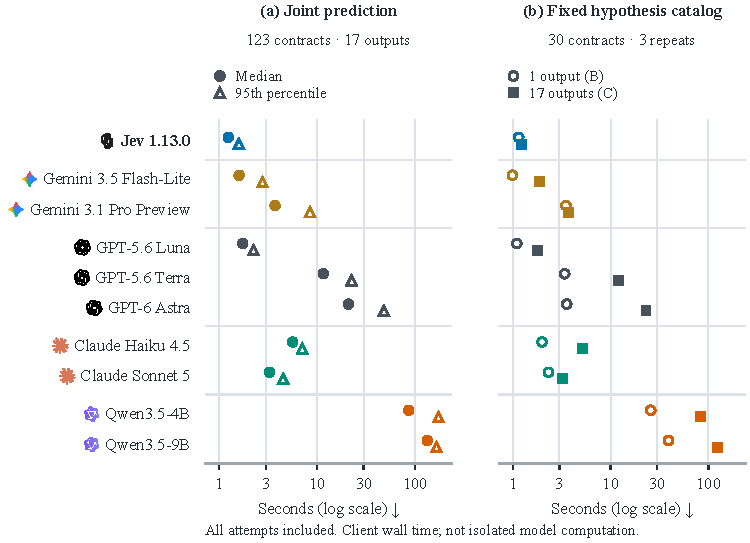
\includegraphics[width=0.90\textwidth]{figures/test_response_time.pdf}
\caption[Jev response time under joint prediction and fixed visible content.]{Jev has the lowest baseline median latency among the tested configurations, with a small additional delay when more judgments are requested. Left: median and 95th-percentile client elapsed time for 123 joint requests per model. Right: median time for requesting one or 17 judgments from the same visible hypothesis catalog (90 requests per condition). All attempts, including invalid responses, are retained. Provider routes and inference settings differ; these measurements do not isolate model computation or establish an architectural cause.
}
\label{fig:testtiming}
\end{figure}

\end{document}
